\documentclass{sintefbeamer}
\usepackage[utf8]{inputenc}
\usepackage[T1]{fontenc}
\usepackage[french]{babel}
\usepackage{adjustbox}

\newtheorem{pro1}{Proposition}
\newtheorem{def1}{Définition}
\newtheorem{exam1}{Exemple}
\newtheorem{theo1}{Théorème}
\newtheorem{pre1}{Preuve}
\newtheorem{rema1}{Remarque}

\uselanguage{French}
\languagepath{French}

\deftranslation[to=French]{Example}{Exemple}
\deftranslation[to=French]{Contents}{Plan}

\makeatletter
\setbeamertemplate{theorem begin}
{
  \begin{\inserttheoremblockenv}
  {%
    \inserttheoremheadfont
    \inserttheoremname
    \ \inserttheoremnumber
    \ifx\inserttheoremaddition\@empty\else\ \inserttheoremaddition\fi%
    \inserttheorempunctuation
  }%
}
\makeatother

% meta-data
\title{Résolution Numérique\\ des Équations Différentielles Fractionnaires}
\subtitle{Méthode de Perturbation d'Homotopie}
\author{\href{mailto:elghemary@gmail.com}{EL GHEMARY Farah}}
\date{20 Juin 2023}
%\titlebackground{images/background}

%% Adding page numbers
\setbeamertemplate{footline}{
    \hfill\usebeamerfont{footline}\insertframenumber/\inserttotalframenumber\hspace*{2ex}
}

% document body
\begin{document}

\maketitle

% INTRODUCTION
\section{Introduction}

\begin{frame}{\hspace{1cm}}
    Les EDFs sont très importantes dans plusieurs domaines comme la physique, l'ingénierie ou encore l'économie. Elles nous aident à représenter des situations complexes, mais il est souvent difficile de les résoudre directement. C'est là que la résolution numérique intervient, nous permettant de trouver des solutions même quand c'est compliqué.
\end{frame}

%CHAPITRE 2
\section{Bases Mathématiques du calcul fractionnaires}

\begin{frame}[fragile]{Pré-requis du calcul ordinaire}
\textbf{Théorème Fondamental de l'Analyse}\\
\begin{equation}\label{FTC}
        \frac{d}{dt}\int_a^t f(t) = f(t) \hspace{1cm} \forall t\in[a,b]
    \end{equation}
\end{frame}


\begin{frame}[fragile]{Fonction Gamma}
\begin{def1}
    On désigne par $\Gamma (x)$ la fonction définie dans l'intervalle $]0,+\infty[$, par l'intégrale généralisée suivant
    \begin{equation}
        \Gamma(x)=\int_{0}^{\infty} e^{-t} t^{x-1}dt.
    \end{equation}
    (seconde intégrale eulérienne)
\end{def1}
\end{frame}


\begin{frame}[fragile]{Fonction Gamma}
\begin{figure}
    \centering
    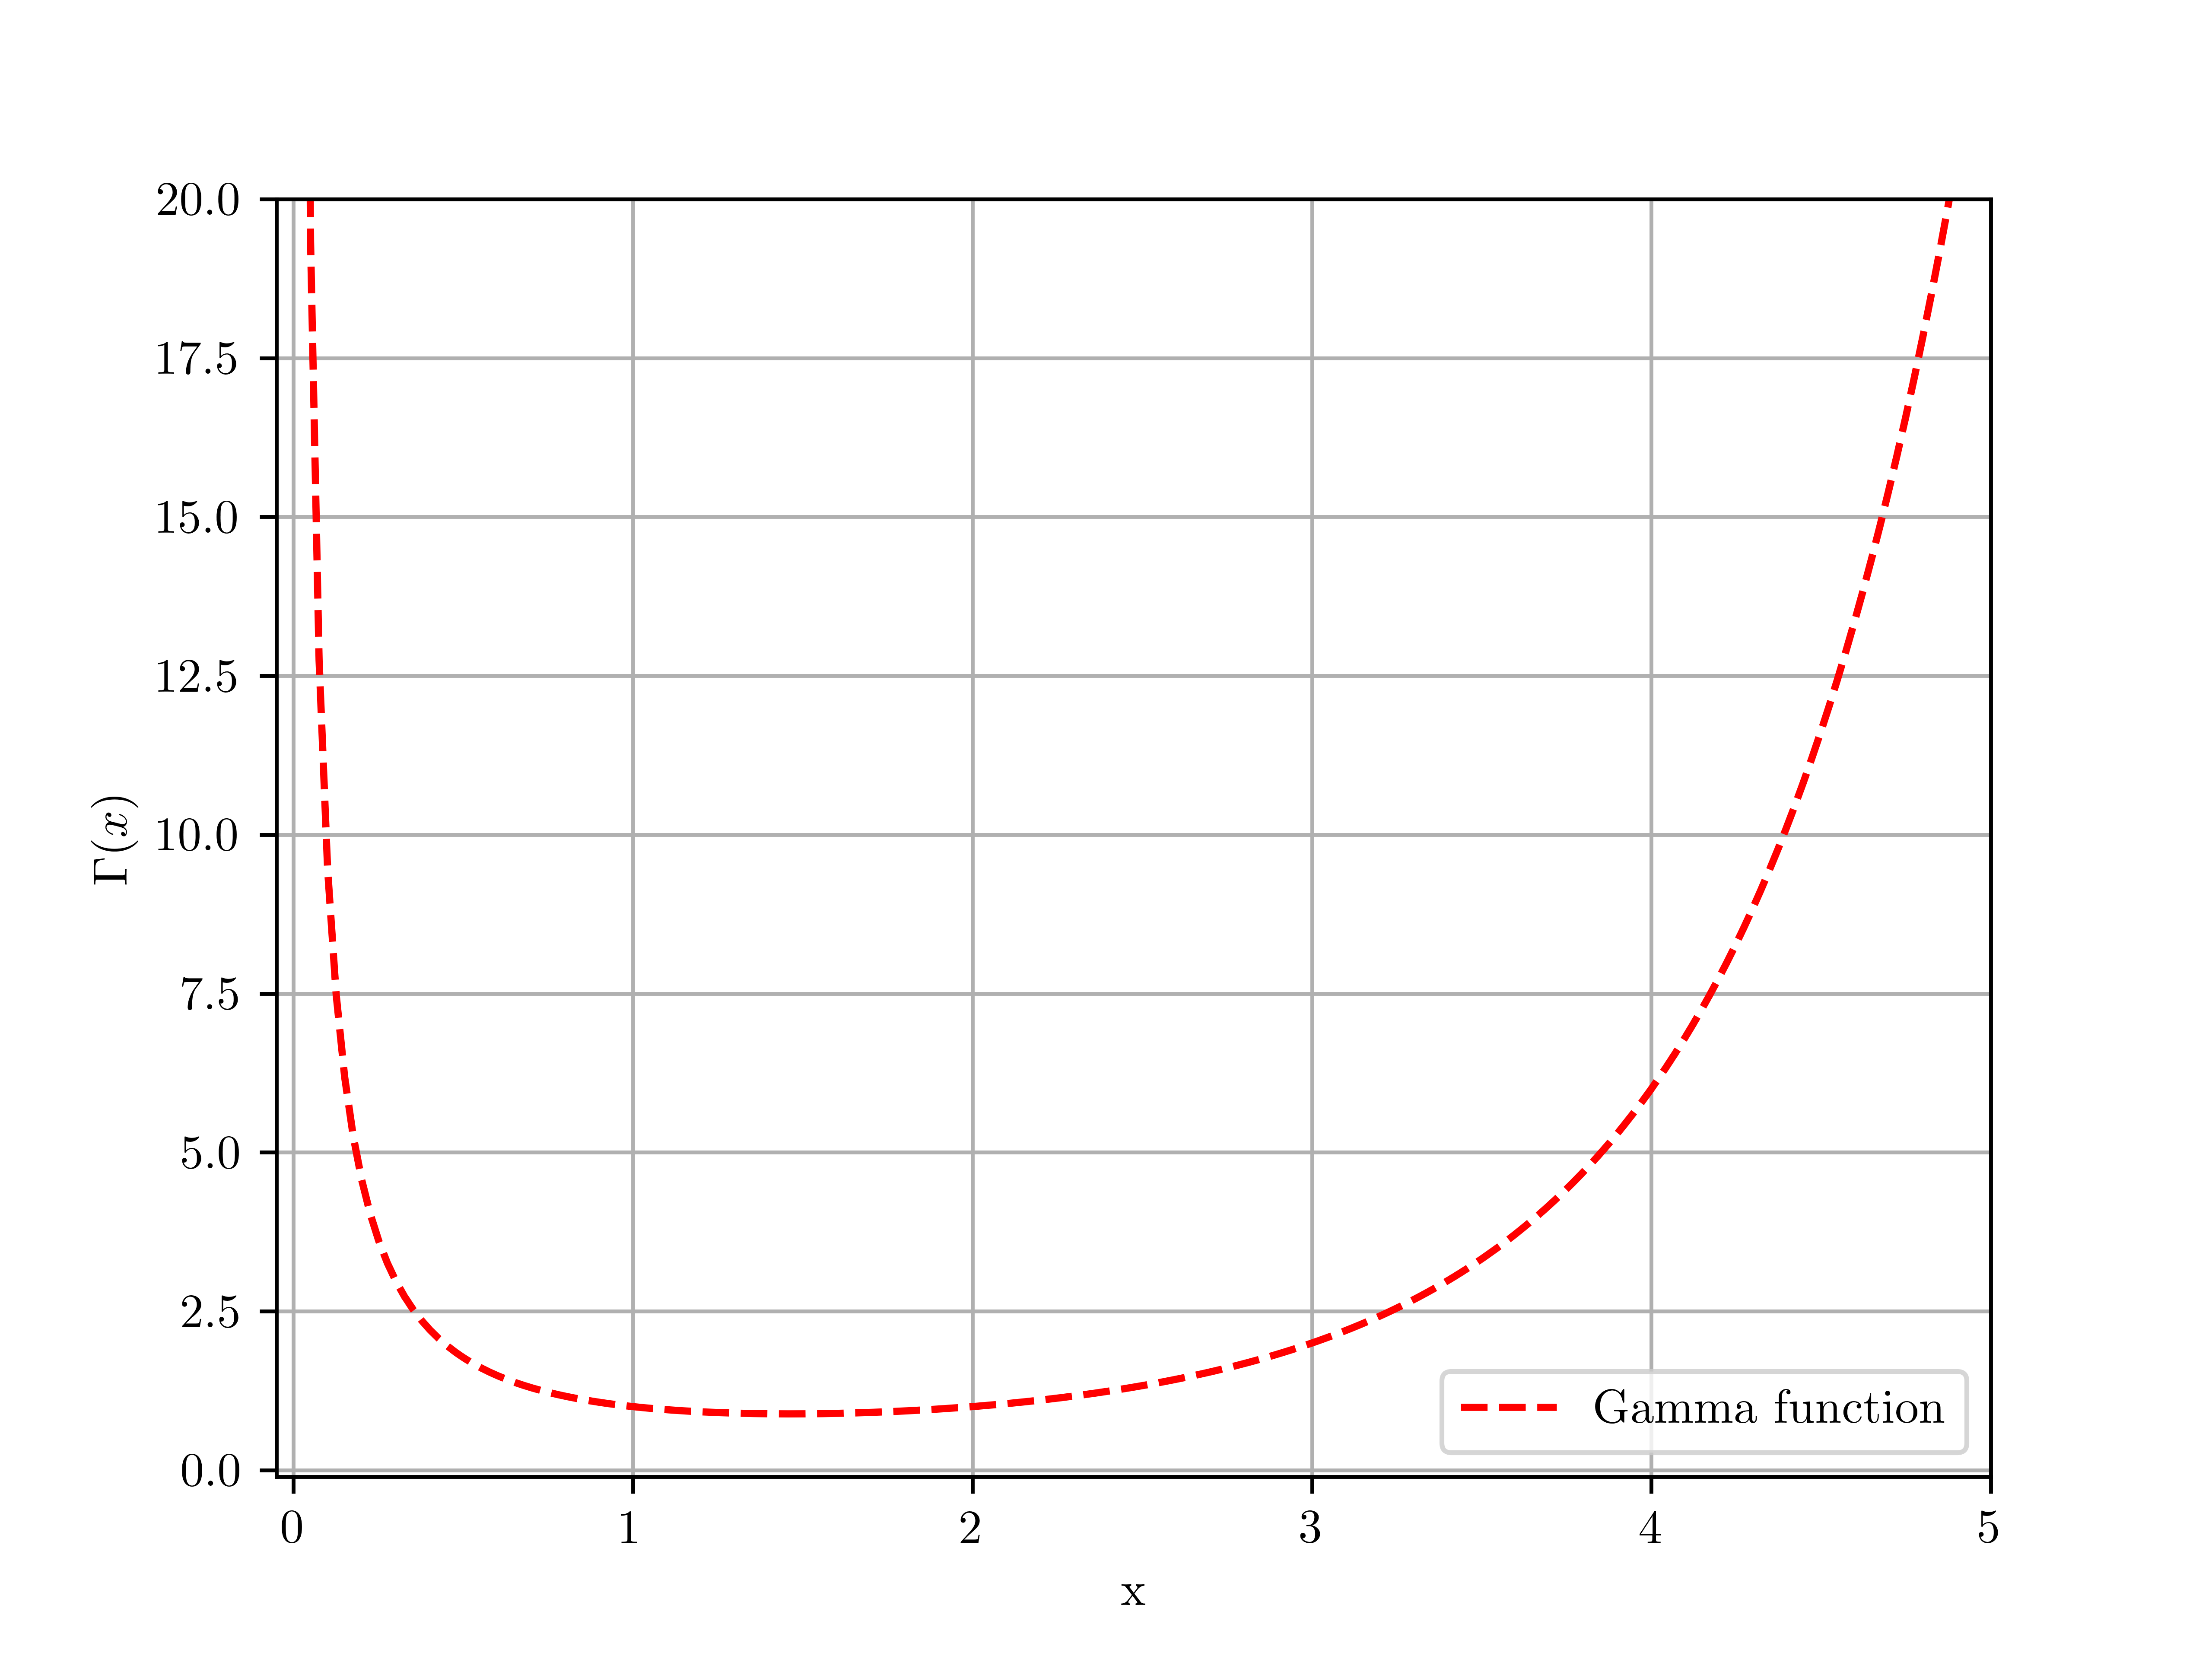
\includegraphics[scale = 0.5]{PolyU Presentation/images/gamma_func.png}
\end{figure}
\end{frame}


\begin{frame}[fragile]{Fonction Gamma}
\begin{example}
    \begin{enumerate}
        \item $\Gamma(1) = 1$
        \item $\Gamma{(\frac{1}{2})} = \sqrt{\pi}$
    \end{enumerate}
\end{example}
\begin{pro1}
    Soient $n\in \mathbb{N}$. On a les identités suivantes:
        \begin{enumerate}
            \item $\Gamma(x+1) = x\Gamma(x)$, pour tout $x > 0$\label{gamma_n}
            \item $\Gamma(x+n) = x(x+1) ... (x+n-1)\Gamma(x)$, \label{gamma_tout_entiers} pour tout $x\in \mathbb{R \textbackslash Z^-}$ tel que $ -n < \Re(x) \leq -n+1 $.
        \end{enumerate}
\end{pro1}
\end{frame}

\begin{frame}{Fonction Gamma}
%\begin{rema1}
    Si on prend $x=1$ dans la propriété (\ref{gamma_tout_entiers}), on obtient $ \Gamma(n+1)=n!, \forall n \in \mathbb{N}.$
%\end{rema1}
\vspace{-0.2cm}
\begin{figure}[H]
    \centering
    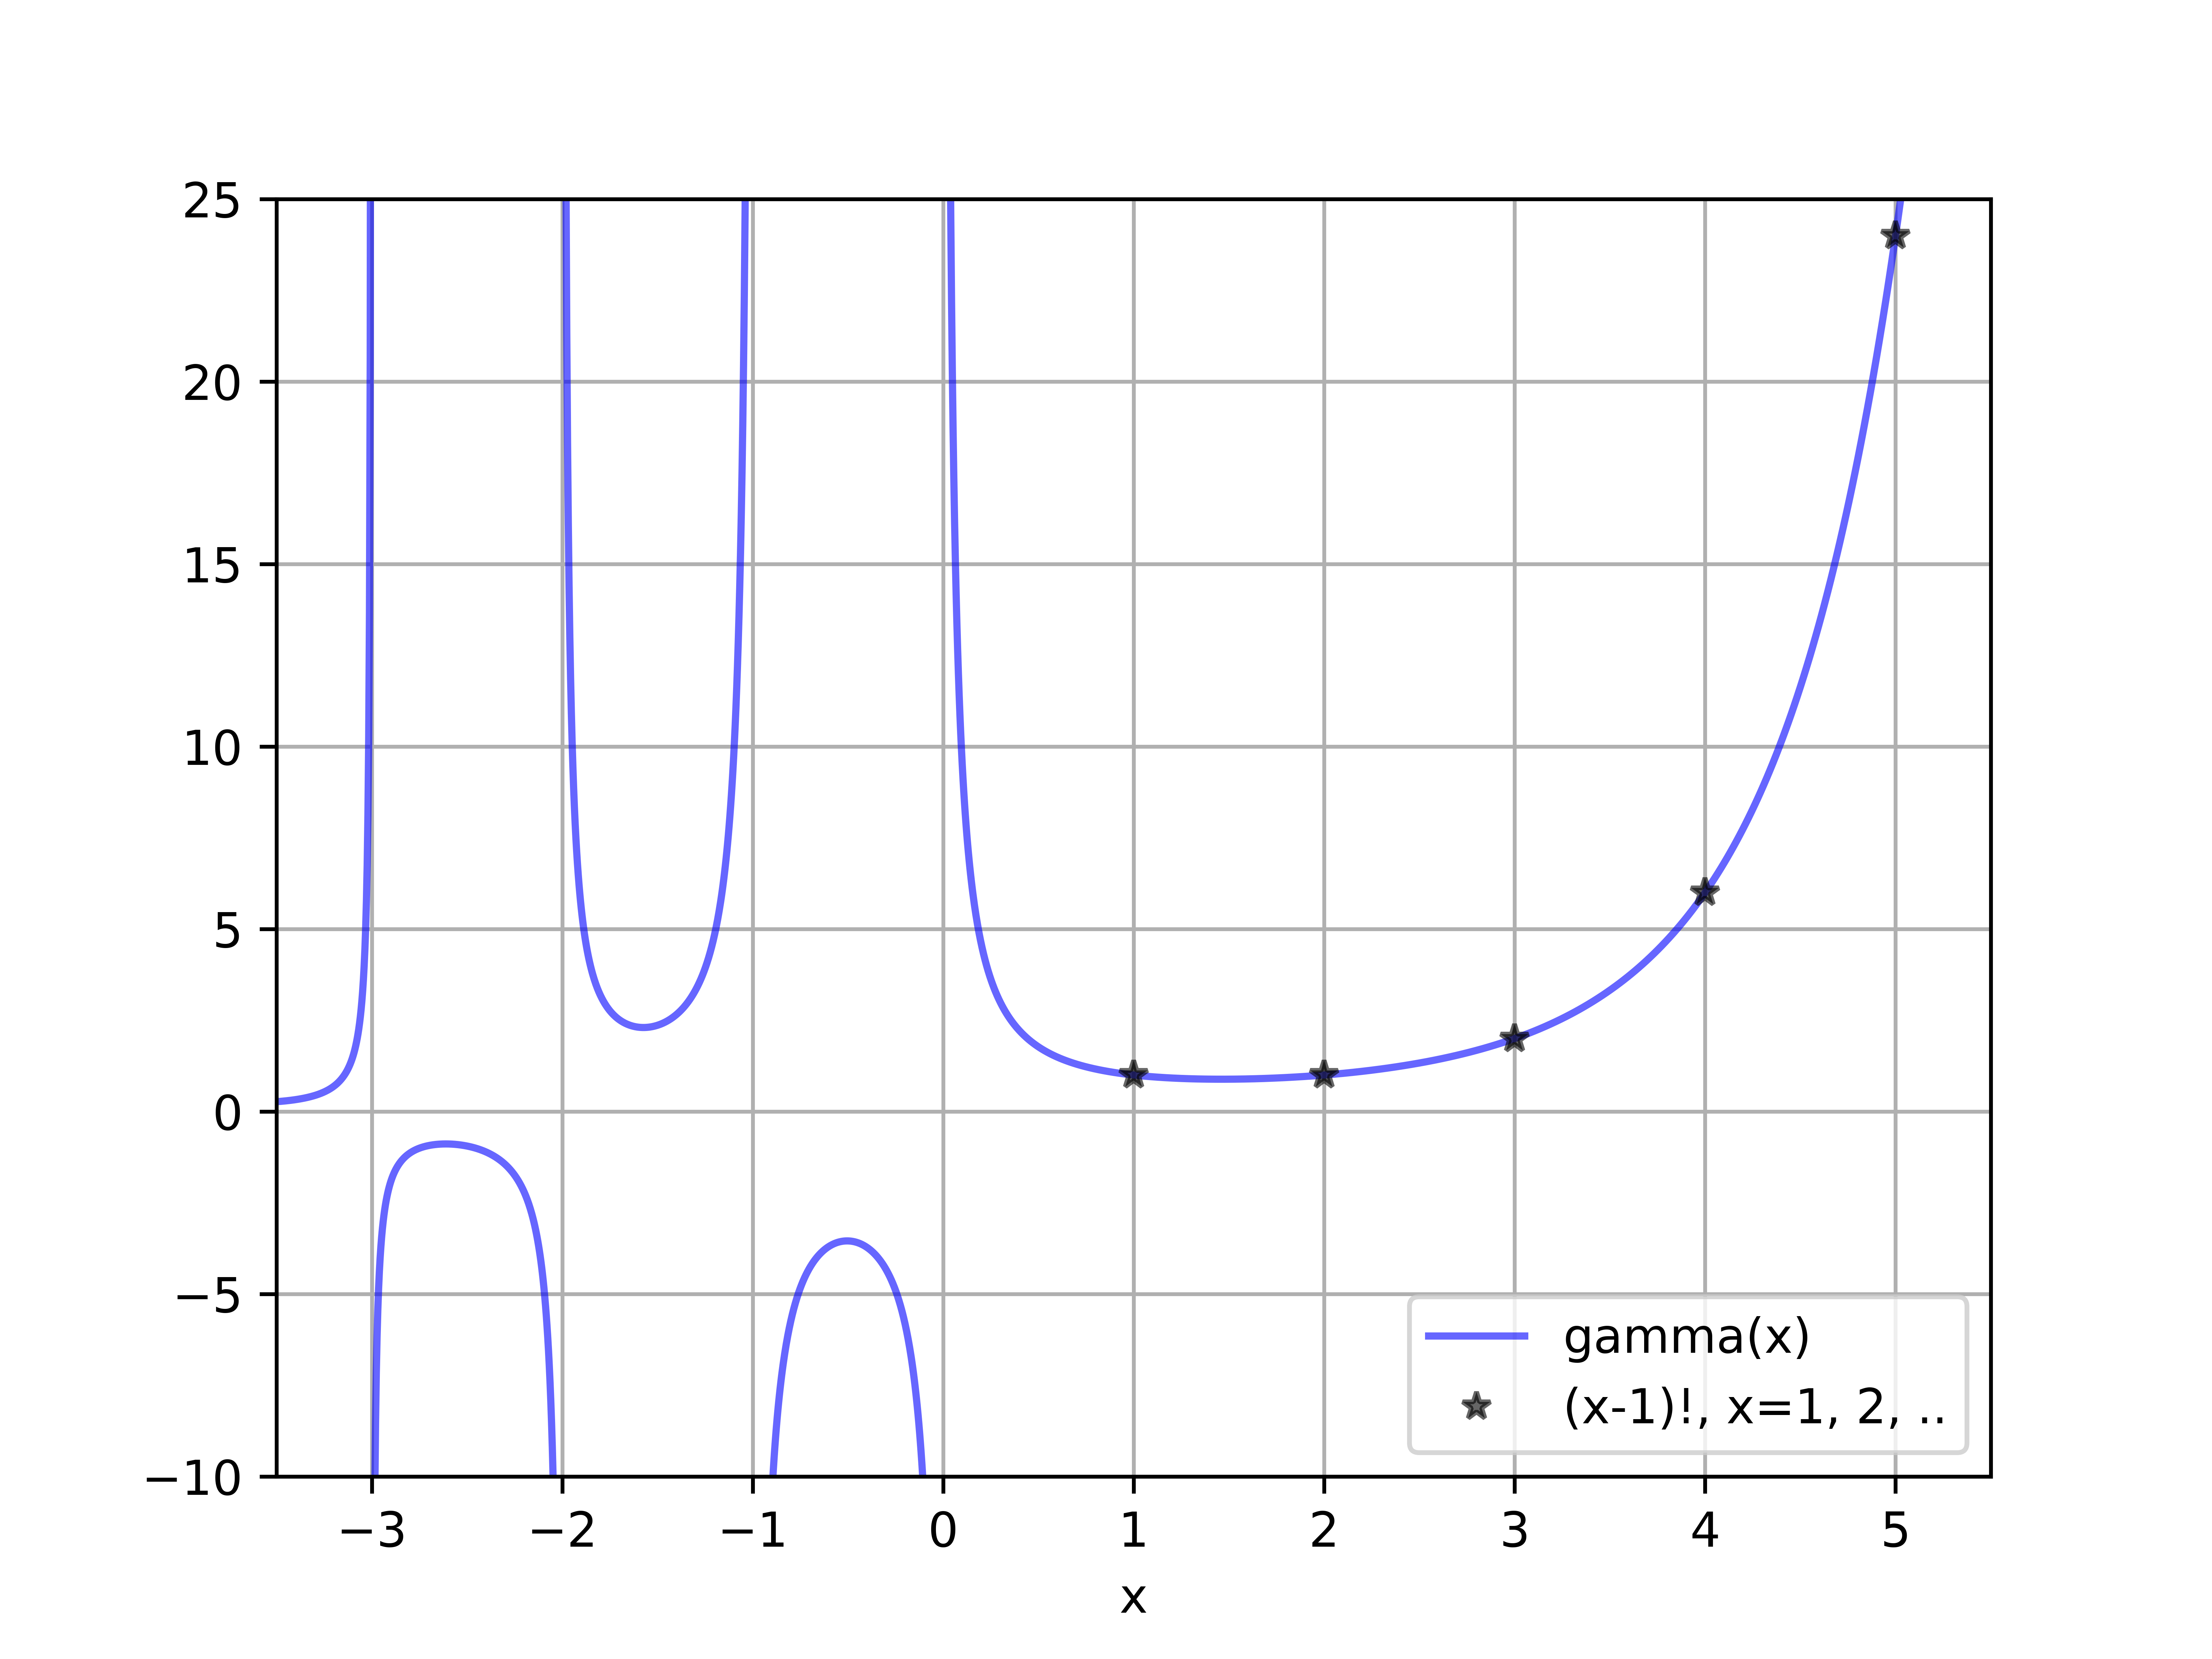
\includegraphics[scale = 0.5]{PolyU Presentation/images/gamma.png}
\end{figure}
\end{frame}


\begin{frame}{Fonction Bêta}
    \begin{def1}
On désigne par $\beta(x,y)$ la fonction définie pour $x>0$ et $y>0$
par l’intégrale suivant:
    \begin{equation}
        \beta(x,y) = \int_{0}^{1} t^{x-1}(1-t)^{y-1} dt
    \end{equation}
    (première intégrale eulérienne)
\end{def1}
\end{frame}


\begin{frame}{Fonction Bêta}
    \begin{theo1}
    La fonction bêta est symétrique, on a
    \begin{equation}
        \beta(x,y)=\beta(y,x)
    \end{equation}
\end{theo1}
\begin{theo1}
    La relation avec la fonction Gamma\\
    \begin{equation}
        \beta(x,y) = \frac{\Gamma(x)\Gamma(y)}{\Gamma(x+y)} = \frac{(x-1)!(y-1)!}{(x+y-1)!}.
    \end{equation}
\end{theo1}
\end{frame}

\begin{frame}{Mittag-Leffler}
    \begin{def1}
    \begin{equation}\label{def:mittag-leffler1}
        E_{\alpha}(x) = \sum _{k=0}^{\infty} \frac{x^k}{\Gamma(\alpha k +1)}, \hspace{1cm} \alpha>0
    \end{equation}
\end{def1}
\begin{example}
    \begin{enumerate}
        \item $E_0(x) = \frac{1}{1-x}$, (somme d'une série géométrique)
        \item $E_1(x) = e^x $, (série exponentielle)
    \end{enumerate}
\end{example}
\end{frame}

\begin{frame}{Fonction Mittag-Leffler}
    \begin{figure}[H]
    \centering
    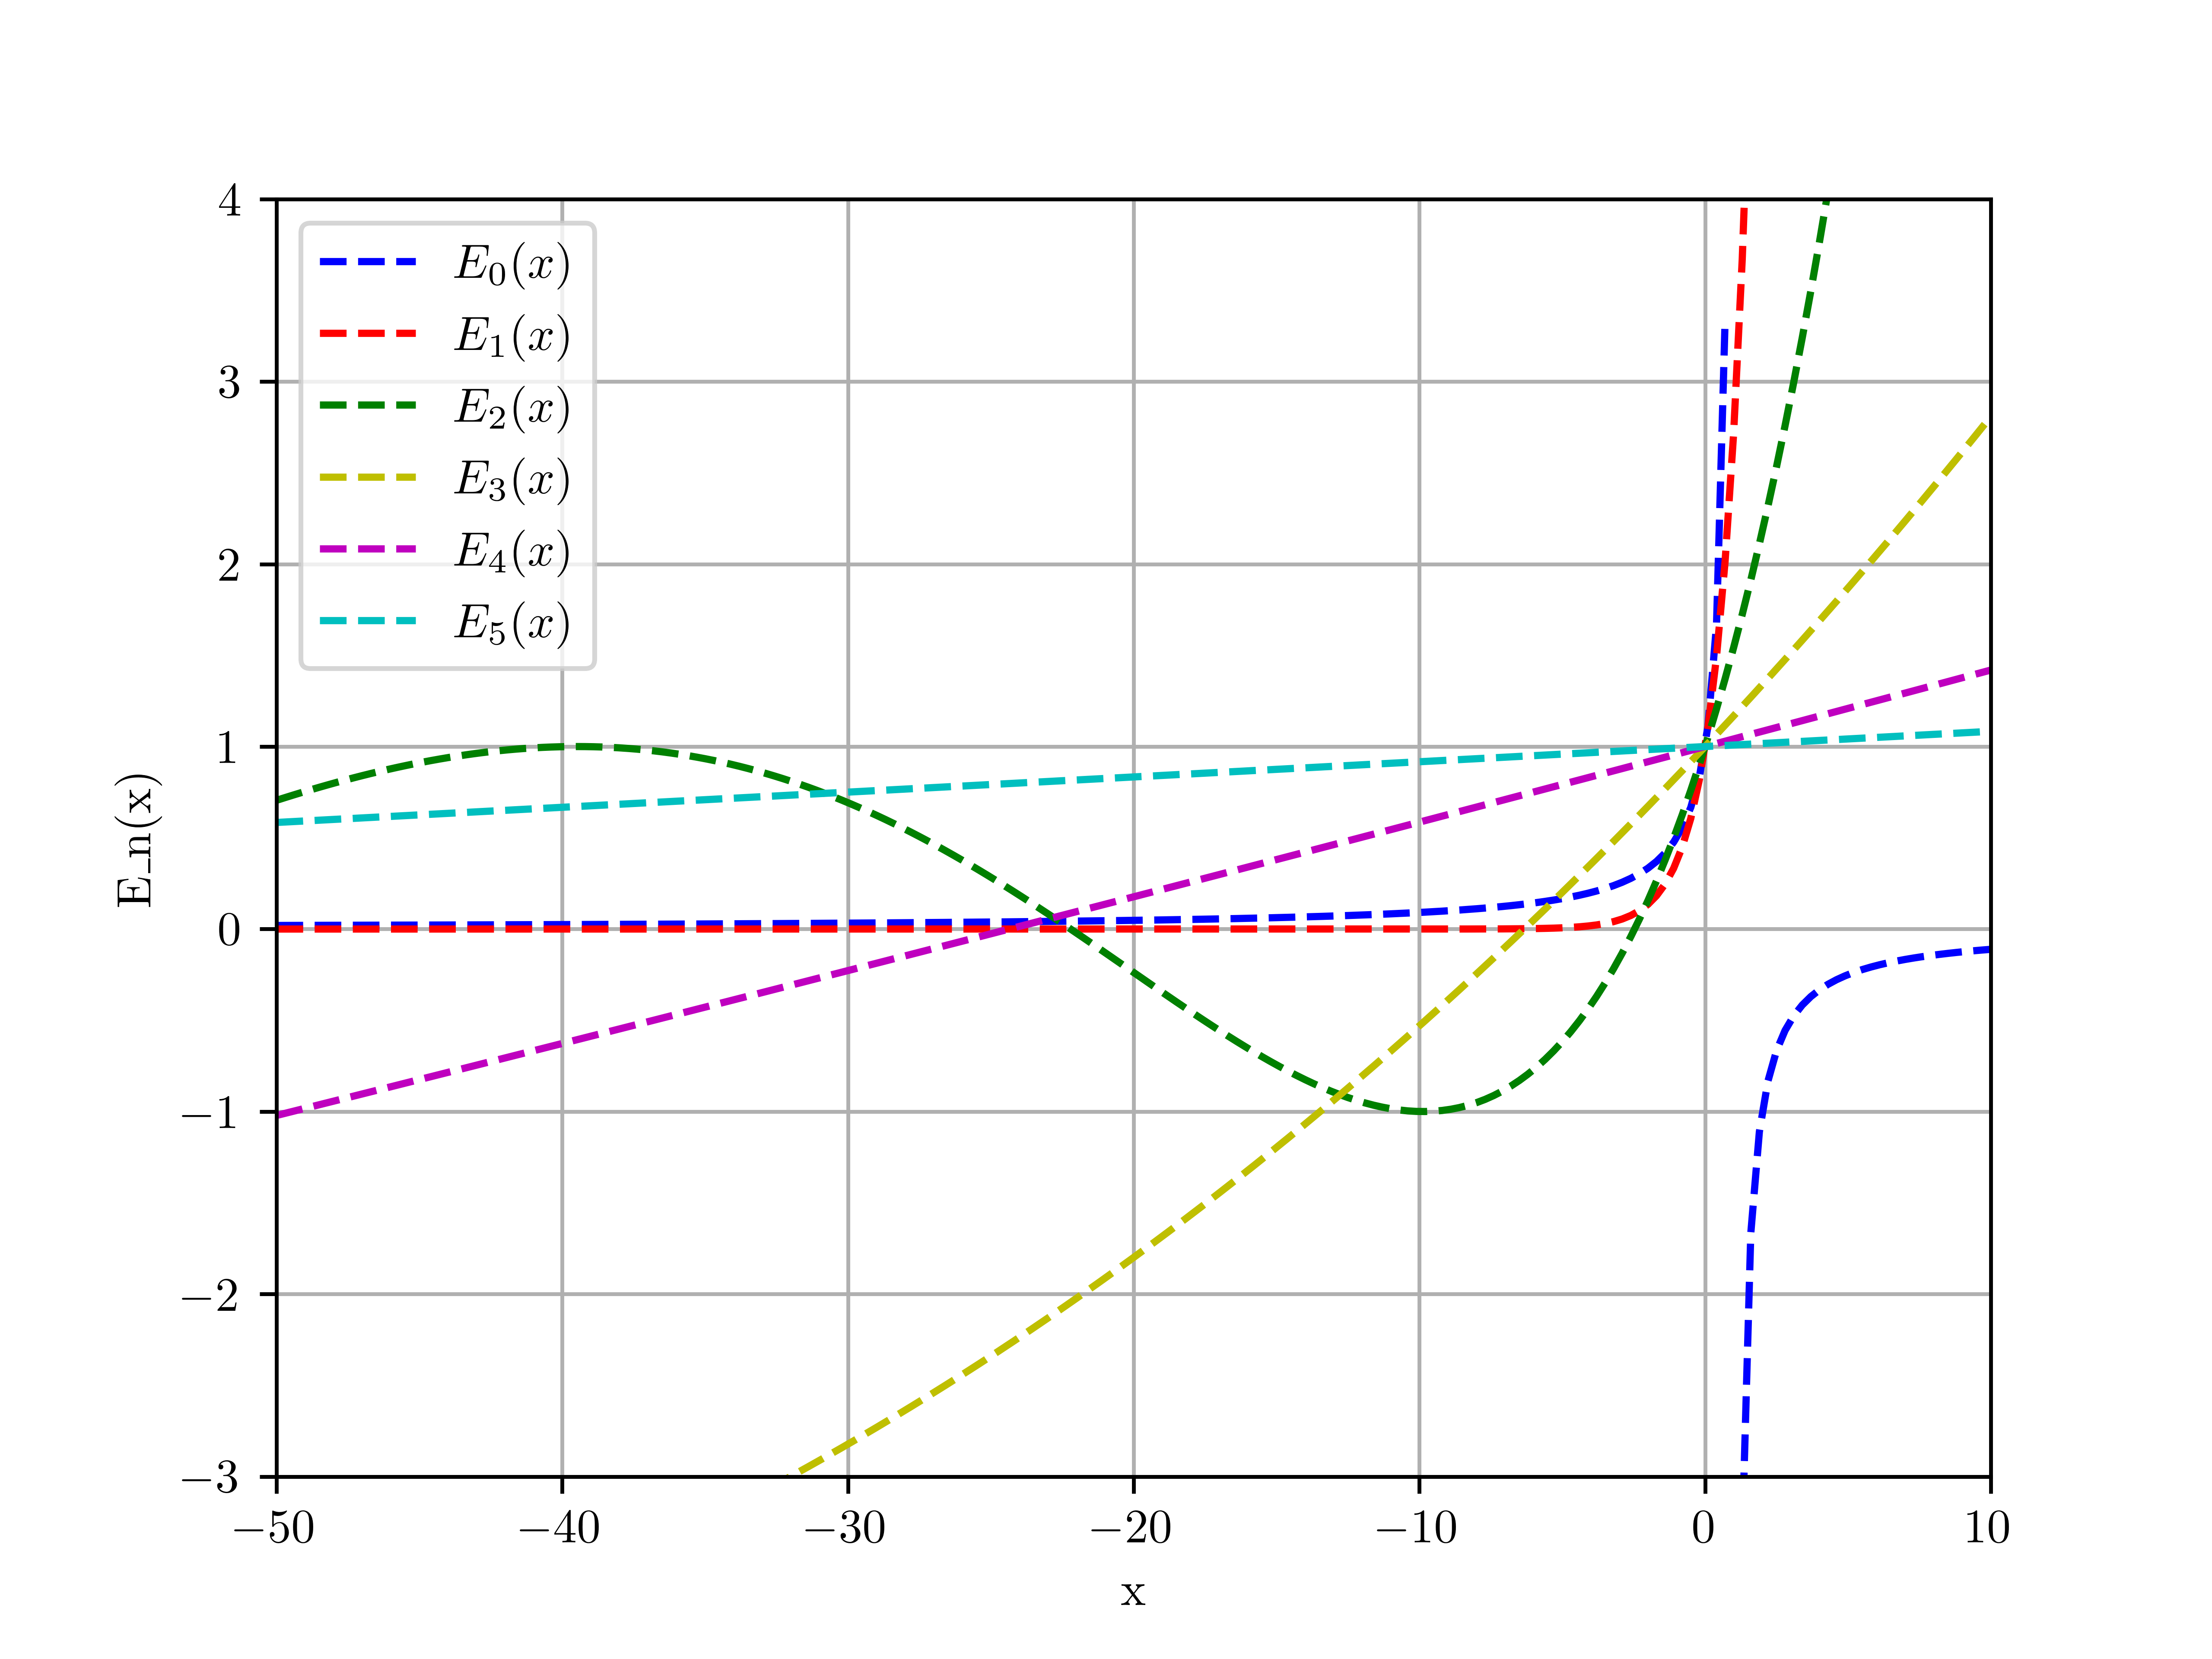
\includegraphics[scale = 0.55]{PolyU Presentation/images/mittag_leffler.png}

\end{figure}
\end{frame}
\begin{frame}{Fonction Mittag-Leffler}
    \begin{def1}
définie par le développement en série suivant:
    \begin{equation}\label{def:mittag-leffler2}
        E_{\alpha, \beta}(x) = \sum _{k=0}^{\infty} \frac{x^k}{\Gamma(\alpha k +\beta)}, \hspace{1cm} \alpha>0, \hspace{0.3cm}\beta>0
    \end{equation}
\end{def1}
\begin{rema1}
    Si $\beta =1$, alors $E_{\alpha, \beta}$ coïncide avec $E_{\alpha}$
    \begin{equation}
        E_{\alpha, 1}=E_{\alpha}
    \end{equation}
\end{rema1}
\begin{example}
        \begin{enumerate}
            \item $E_{1,1} (x)= e^x$,
            \item $E_{1,2}(x) = \frac{e^x - 1}{x}$
        \end{enumerate}
    \end{example}
\end{frame}


% CHAPITRE 3
\section{Éléments du calcul fractionnaire}

\begin{frame}{Intégrale fractionnaire au sens de Riemann-Liouville}
le formule de Cauchy pour le n-ème intégral :
\begin{equation} \label{eq:int_succ}
    I_{a}^{n} f(t) = \int_{a}^{t} \int_{a}^{\tau_{n-1}} ... \int_{a}^{\tau_1} f(\tau) d\tau d\tau_1 ... d\tau_{n-1} = \frac{1}{(n-1)!}\int_{a}^{t} (t-\tau)^{n-1} f(\tau)d\tau
\end{equation}
    \begin{def1}
         L'intégrale fractionnaire de Riemann-Liouville d'ordre $\alpha \in \mathbb{R^+}$ d'une fonction $f\in \textbf{L}^1 [a,b]$ est définie par:
    \begin{equation}\label{eq:integraleR-L}
        I_{a}^{\alpha} f(t) = {}_a^{RL} D_t^{-\alpha} f(t) =\frac{1}{\Gamma(\alpha)} \int_{a}^{t} (t-s)^{\alpha-1} f(s) ds.
    \end{equation}
    \end{def1}
\end{frame}

\begin{frame}{Intégrale fractionnaire au sens de Riemann-Liouville}
\textbf{Fonctions usuelles}
\begin{itemize}
    \item Fonction puissance: $f(t)=(t-a)^\beta$, \hspace{0.3cm} $t\in[a,b]$, \hspace{0.3cm} $a\in\mathbb{R}$ \hspace{0.3cm} et $\beta > -1$. \\
\begin{equation} \label{eq:I_R-L_fct_puissance}
    I_{a}^{\alpha} (t-a)^\beta=\frac{\Gamma(\beta +1)}{\Gamma(\beta + \alpha + 1)}(t-a)^{\beta + \alpha}.
    \end{equation}
    \end{itemize}
\end{frame}



\begin{frame}{Intégrale fractionnaire au sens de Riemann-Liouville}
    \begin{itemize}
        \item Fonction constante: $f(t) =C \in \mathbb{R}$ est une constante. Alors 
\begin{equation} \label{integral_R-L}
    I_{a}^{\alpha} C= \frac{C}{\Gamma(\alpha + 1)}(t-a)^\alpha
\end{equation}
\item Fonction exponentielle: $f(t) = e^{kt}$, où $k\in \mathbb{R}$ est une constante
\begin{equation}
    I_{a}^{\alpha} e^{kt}=\frac{1}{\Gamma(\alpha)} \int_{0}^{t-a} s^{\alpha - 1}e^{k(t-s)} ds.
\end{equation}
    \end{itemize}
\end{frame}

\begin{frame}{Intégrale fractionnaire au sens de Riemann-Liouville}
    \textbf{Propriétés:}
    \begin{itemize}
        \item Soient $f \in C[a,b]$ $\beta >0$, et $\alpha >0$. Alors on a 
    \begin{equation}
        I_{a}^{\alpha}[I_{a}^{\beta}f(t)] = I_{a}^{\alpha + \beta} f(t)
    \end{equation}
    \item Pour tout $\alpha, \beta >0$ et $f$ Lebesgue-intégrable sur $[a,b]$ on a :
    \begin{equation}
        \frac{d^k}{dt^k}[I_a^{\alpha} f(t)] = I_{a}^{\alpha - k} f(t) , \hspace{1cm} \alpha >1, \hspace{1cm}\forall k <\alpha.
    \end{equation}
    \item Soient $f$ fonction continue sure $[0,b[$. Si $Df$ est continue alors pour tout $t>0$ on a :
    \begin{equation}
        D[I_{a}^{\alpha}f(t)] = I_{a}^{\alpha}[Df(t)]+\frac{f(0)}{\Gamma(\alpha)}t^{n-\alpha}
    \end{equation}
    \end{itemize}
\end{frame}


\begin{frame}{Dérivée fractionnaire au sens de Riemann-Liouville}
    \begin{definition}
    La dérivée fractionnaire au sens de Riemann-Liouville d'ordre $\alpha$ de la fonction $f$, notée $ \textbf{D}_a^{\alpha}$, est la fonction définie par :\\
    \begin{equation} \label{eq:D_R-L}
        \textbf{D}_a^{\alpha} = \frac{d^n}{dt^n} \left[I_a^{n-\alpha} f(t) \right],
    \end{equation}
    avec $n =[\alpha] + 1$ où $[.]$ est la partie entière. 
    De manière équivalente, nous avons:
\begin{equation}
    \textbf{D}_a^{\alpha} =
        \frac{1}{\Gamma(n-\alpha)} \frac{d^n}{dt^n}\left( \int_a^t(t-s)^{n-\alpha-1}f(s)ds\right) \hspace{1cm} n-1<\alpha<n, \hspace{0.3cm} n\in\mathbb{N^*}
\end{equation}
\end{definition}
\end{frame}

\begin{frame}{Dérivée fractionnaire au sens de Riemann-Liouville}
    \textbf{Fonctions usuelles :}
    \begin{itemize}
        \item Fonction puissance : $g(t)=(t-a)^\gamma$, et $0<n-1<\alpha<n$ avec $\gamma > n-1$ on a alors:
        \begin{equation}
            \textbf{D}_a^{\alpha} (t-a)^{\gamma}=\frac{\Gamma(\gamma+1)}{\Gamma(\gamma - \alpha +1)}(t-a)^{\gamma - \alpha}
        \end{equation} 
        \item Fonction Constante: $g(t) =C \in \mathbb{R}$ est une constante. Alors 
\begin{equation}
    \textbf{D}_a^{\alpha} C=\frac{C}{\Gamma(1-\alpha)}(t-a)^{-\alpha}.
\end{equation}
    \end{itemize}
\end{frame}

\begin{frame}{Dérivée fractionnaire au sens de Riemann-Liouville}
    \textbf{Propriétés}
    \begin{itemize}
        \item Linéarité : \begin{equation}
    \textbf{D}_a^{\alpha}(\lambda f(t) + \gamma g(t)) = \lambda\textbf{D}_a^{\alpha} f(t) +\gamma\textbf{D}_a^{\alpha} g(t).
\end{equation}
\item Pour $\alpha>0$ et $t>a$, nous avons :
\begin{equation}
    \textbf{D}_a^{\alpha}\left(I_a^{\alpha}f(t)\right) = f(t)
\end{equation}
\item Pour $\alpha \geq 0$ et $\beta \geq 0$, nous avons
\begin{equation*}
    \textbf{D}_a^{\alpha}\left(I_a^{\beta} f(t)\right) = \textbf{D}_a^{\alpha - \beta} f(t)
\end{equation*}
\item Pour $n \leq n-1 \leq \alpha < n$, $n\in \mathbb{N^*}$,
\begin{equation}
    \frac{d^k}{dt^k} \left( \textbf{D}_a^{\alpha} f(t) \right) = \textbf{D}_a^{k+\alpha} f(t),
\end{equation}
    \end{itemize}
\end{frame}

\begin{frame}{Dérivée fractionnaire au sens de Caputo}
    \begin{definition}
    La dérivée fractionnaire de Caputo est définie par:
    \begin{equation}\label{eq:der_frac_caputo}
        D_a^{\alpha} f(t) = I_a^{m-\alpha}\left(\frac{d^m}{dt^m} f(t) \right) = \frac{1}{\Gamma(m-\alpha)}\int_a^t (t-\tau)^{m-\alpha -1} f^{(m)} (s)ds,
    \end{equation}
    pour $m-1\leq\alpha<m$, $m\in \mathbb{N}$, $t>a$
\end{definition}
\end{frame}
\begin{frame}{Dérivée fractionnaire au sens de Caputo}
    \textbf{Fonctions usuelles}
    \begin{itemize}
        \item Fonction puissance: $g(t)=(t-a)^\gamma$,\\
Soient $ 0 < m-1 < \alpha < m$, avec $\gamma > m-1$, alors 
\begin{equation*}
    D_a^{\alpha}(t-a)^{\gamma} = \frac{\Gamma(\gamma+1)}{\Gamma(\gamma-\alpha+1)}(t-a)^{\gamma - \alpha}.
\end{equation*}
\item Fonction Constante : $g(t) =C \in \mathbb{R}$ est une constante. \begin{equation*}
    D_a^{\alpha} C = 0.
\end{equation*} 
    \end{itemize}
    \textbf{Propriétés:}
    \begin{itemize}
        \item Linéarité: Soient $\lambda$, $\gamma \in \mathbb{R}$
\begin{equation}
    D_a^{\alpha}(\lambda f(t)+\gamma g(t))=\lambda D_a^{\alpha}f(t) + \gamma D_a^{\alpha}g(t).
\end{equation}
\end{itemize}
\end{frame}

\begin{frame}{Dérivée fractionnaire au sens de Caputo}
    \begin{itemize}

\item Pour $0\leq m-1<\alpha<m$ et $f$ une fonction telle que $D_a^{\alpha}$ et $\textbf{D}_a^{\alpha}$ existent. Alors 
\begin{equation}
    D_a^{\alpha} f(t) = \textbf{D}_a^{\alpha}f(t) -\sum_{k=0}^{m-1} \frac{f^{(k)}(a)(t-a)^{k-\alpha}}{\Gamma(k-\alpha+1)}.
\end{equation}
    \item Si $f$ est continue, alors
\begin{equation*}
    D_a^{\alpha}(I_a^{\alpha} f(t))=f(t),
\end{equation*}
et \begin{equation*}
    I_a^{\alpha}\left(D_a^{\alpha} f(t) \right)=f(t)-\sum_{k=0}^{m-1} \frac{f^{(k}(a)(t-a)^k}{k!}.
\end{equation*}
\item Soient $n\in\mathbb{N}$ et $m-1\leq\alpha<m$, alors:
\begin{equation}\label{eq:comp_o_n}
    D_a^{\alpha}(D_a^n f(t)) = d_a^{\alpha+n}f(t),
\end{equation}
    \end{itemize}
\end{frame}


%CHAPITRE 4

\begin{frame}{Application de la méthode aux équations différentielles ordinaires}
    \textbf{Description de la méthode} :\\
Soient X et Y deux espaces topologiques. On dit que deux applications continues $f,g:X\mapsto Y$ sont homotopiques s'il existe une application continue :
\begin{align*}
    F:X \times [0,1] & \mapsto Y \\
    (x,p) &\mapsto F(x,p)
\end{align*}
telle que:
\begin{equation*}
    F(x,0)=f(x)
\end{equation*}
et
\begin{equation*}
    F(x,1) = g(x)
\end{equation*}
\end{frame}

\begin{frame}{Application de la méthode aux équations différentielles ordinaires}
    Soit l'équation différentielle non linéaire suivante:
\begin{equation} \label{eq:def_ED}
    A(u)-f=0, \hspace{1cm} r\in\Omega
\end{equation}
avec les conditions aux limites:
\begin{equation}
    B(u,\frac{\partial u}{\partial n}) = 0, \hspace{1cm} r\in \Gamma
\end{equation}
où $A$ est un opérateur différentiel général, $B$ opérateur limite, $f$ est une fonction connue et $\Gamma$ est la frontière de $\Omega$.\\
\end{frame}


\begin{frame}{Application de la méthode aux équations différentielles ordinaires}
     $A$ peut être écrit sous la forme $A=L+N$, où $L $ désigne un opérateur linéaire et $N$ un opérateur non linéaire, alors l'équation \ref{eq:def_ED} devient: 
\begin{equation}
    L(u) + N(u) - f =0
\end{equation}
Construisons maintenant une homotopie $v(r,p): \Omega \times[0,1] \mapsto \mathbb{R}$, qui satisfait:
\begin{equation}\label{eq:sol_hom1}
    H(v,p)=(1-p)[L(v)-L(u_0)]+p[A(v)-f]=0, \hspace{1cm} p\in [0,1],
\end{equation}
où
\begin{equation}\label{eq:sol_hom2}
    H(v,p) = L(v)-L(u_0) +pL(u_0)+p[N(v)-f]=0,
\end{equation}
\end{frame}


\begin{frame}{Application de la méthode aux équations différentielles ordinaires}
    Les formules \ref{eq:sol_hom1} et \ref{eq:sol_hom2} impliquent:
    \begin{equation}
        H(v,0)=L(v)-L(u_0)=0,
    \end{equation}
    \begin{equation}
        H(v,1)=A(v)-f=0,
    \end{equation}
    supposons que la solution de \ref{eq:sol_hom1} et \ref{eq:sol_hom2} sont exprimées comme:
    \begin{equation}
        v=v_0+pv_1+p^2v_2+p^3v_3+ .... = \sum_{i=0}^{\infty}v_ip^i
    \end{equation}
    La solution analytique approché de l'équation \ref{eq:def_ED} est donnée par :
    \begin{equation}
        u=\lim_{p\mapsto1}v = v_0 + v_1+v_2 +...
    \end{equation} 
\end{frame}



\begin{frame}{Application de la méthode aux équations différentielles ordinaires}
    \textbf{Application: Exemple 1} \\
    Considérons l'équation différentielle non linéaire suivante:
\begin{equation} \label{ex:EDO_1}
    \begin{cases}
        u'(t)+u^2(t)=0, \hspace{1cm} t\geq 0,\\
        u(0)=1,
    \end{cases}
\end{equation}
où la solution exact est donnée par:
\begin{equation}
    u(t)=\frac{1}{1+t}.
\end{equation}
\end{frame}


\begin{frame}{Application de la méthode aux équations différentielles ordinaires}
     On construit l'homotopie suivante :
\begin{equation*}
    H: \Omega\times[0,1] \mapsto\mathbb{R}
\end{equation*}
\begin{align}
    (1-p)\left(v'(t)-u'_0(t)\right)+p\left(v'(t)+v^2 (t)\right), \hspace{0.5cm} p\in[0,1], \hspace{0.5cm} t\in \Omega
\end{align}
avec $u_0=u(0)=1$.\\
La solution de l'équation \ref{ex:EDO_1} peut être exprimée comme suit:
\begin{equation}\label{sol:EDO_1}    v=v_0+pv_1+p^2v_2+p^3v_3...=\sum_{k=0}^{\infty} p^{k}v_k.
\end{equation}
\end{frame}


\begin{frame}{Application de la méthode aux équations différentielles ordinaires}
    Substituons l'équation \ref{sol:EDO_1} dans l'équation \ref{ex:EDO_1} et identifions les termes de même puissance de $p$, il vient:
\begin{align*}
    \begin{cases}
        &p^0 : v'_0(t) = u'_0(t),\\
        &p^1 : v'_1(t) = u'_0(t)-v^2_0(t), \hspace{1cm} v_1(0)=0,\\
        &p^2 : v'_2(t) = -2v_0(t)v_1(t), \hspace{1cm} v_2(t)=0,\\
        &    .\\
        &    .\\
        &    .\\
    \end{cases}
\end{align*}
\end{frame}


\begin{frame}{Application de la méthode aux équations différentielles ordinaires}
    Par conséquent, nous obtenons:
\begin{align*}
    &v_0(t)=1,\\
    &v_1(t)=-t,\\
    &v_2(t)=t^2.
\end{align*}
    Finalement, la solution approchée de l'équation \ref{ex:EDO_1} est donnée par :
    \begin{equation}
    u(t)=\lim_{p \to 1} v(t) = v_0(t)+v_1(t)+v_2(t) + ... = 1-t + t^2 ...
\end{equation}
\end{frame}


\begin{frame}{Application de la méthode aux équations différentielles ordinaires}
    \begin{figure}[H]
    \centering
    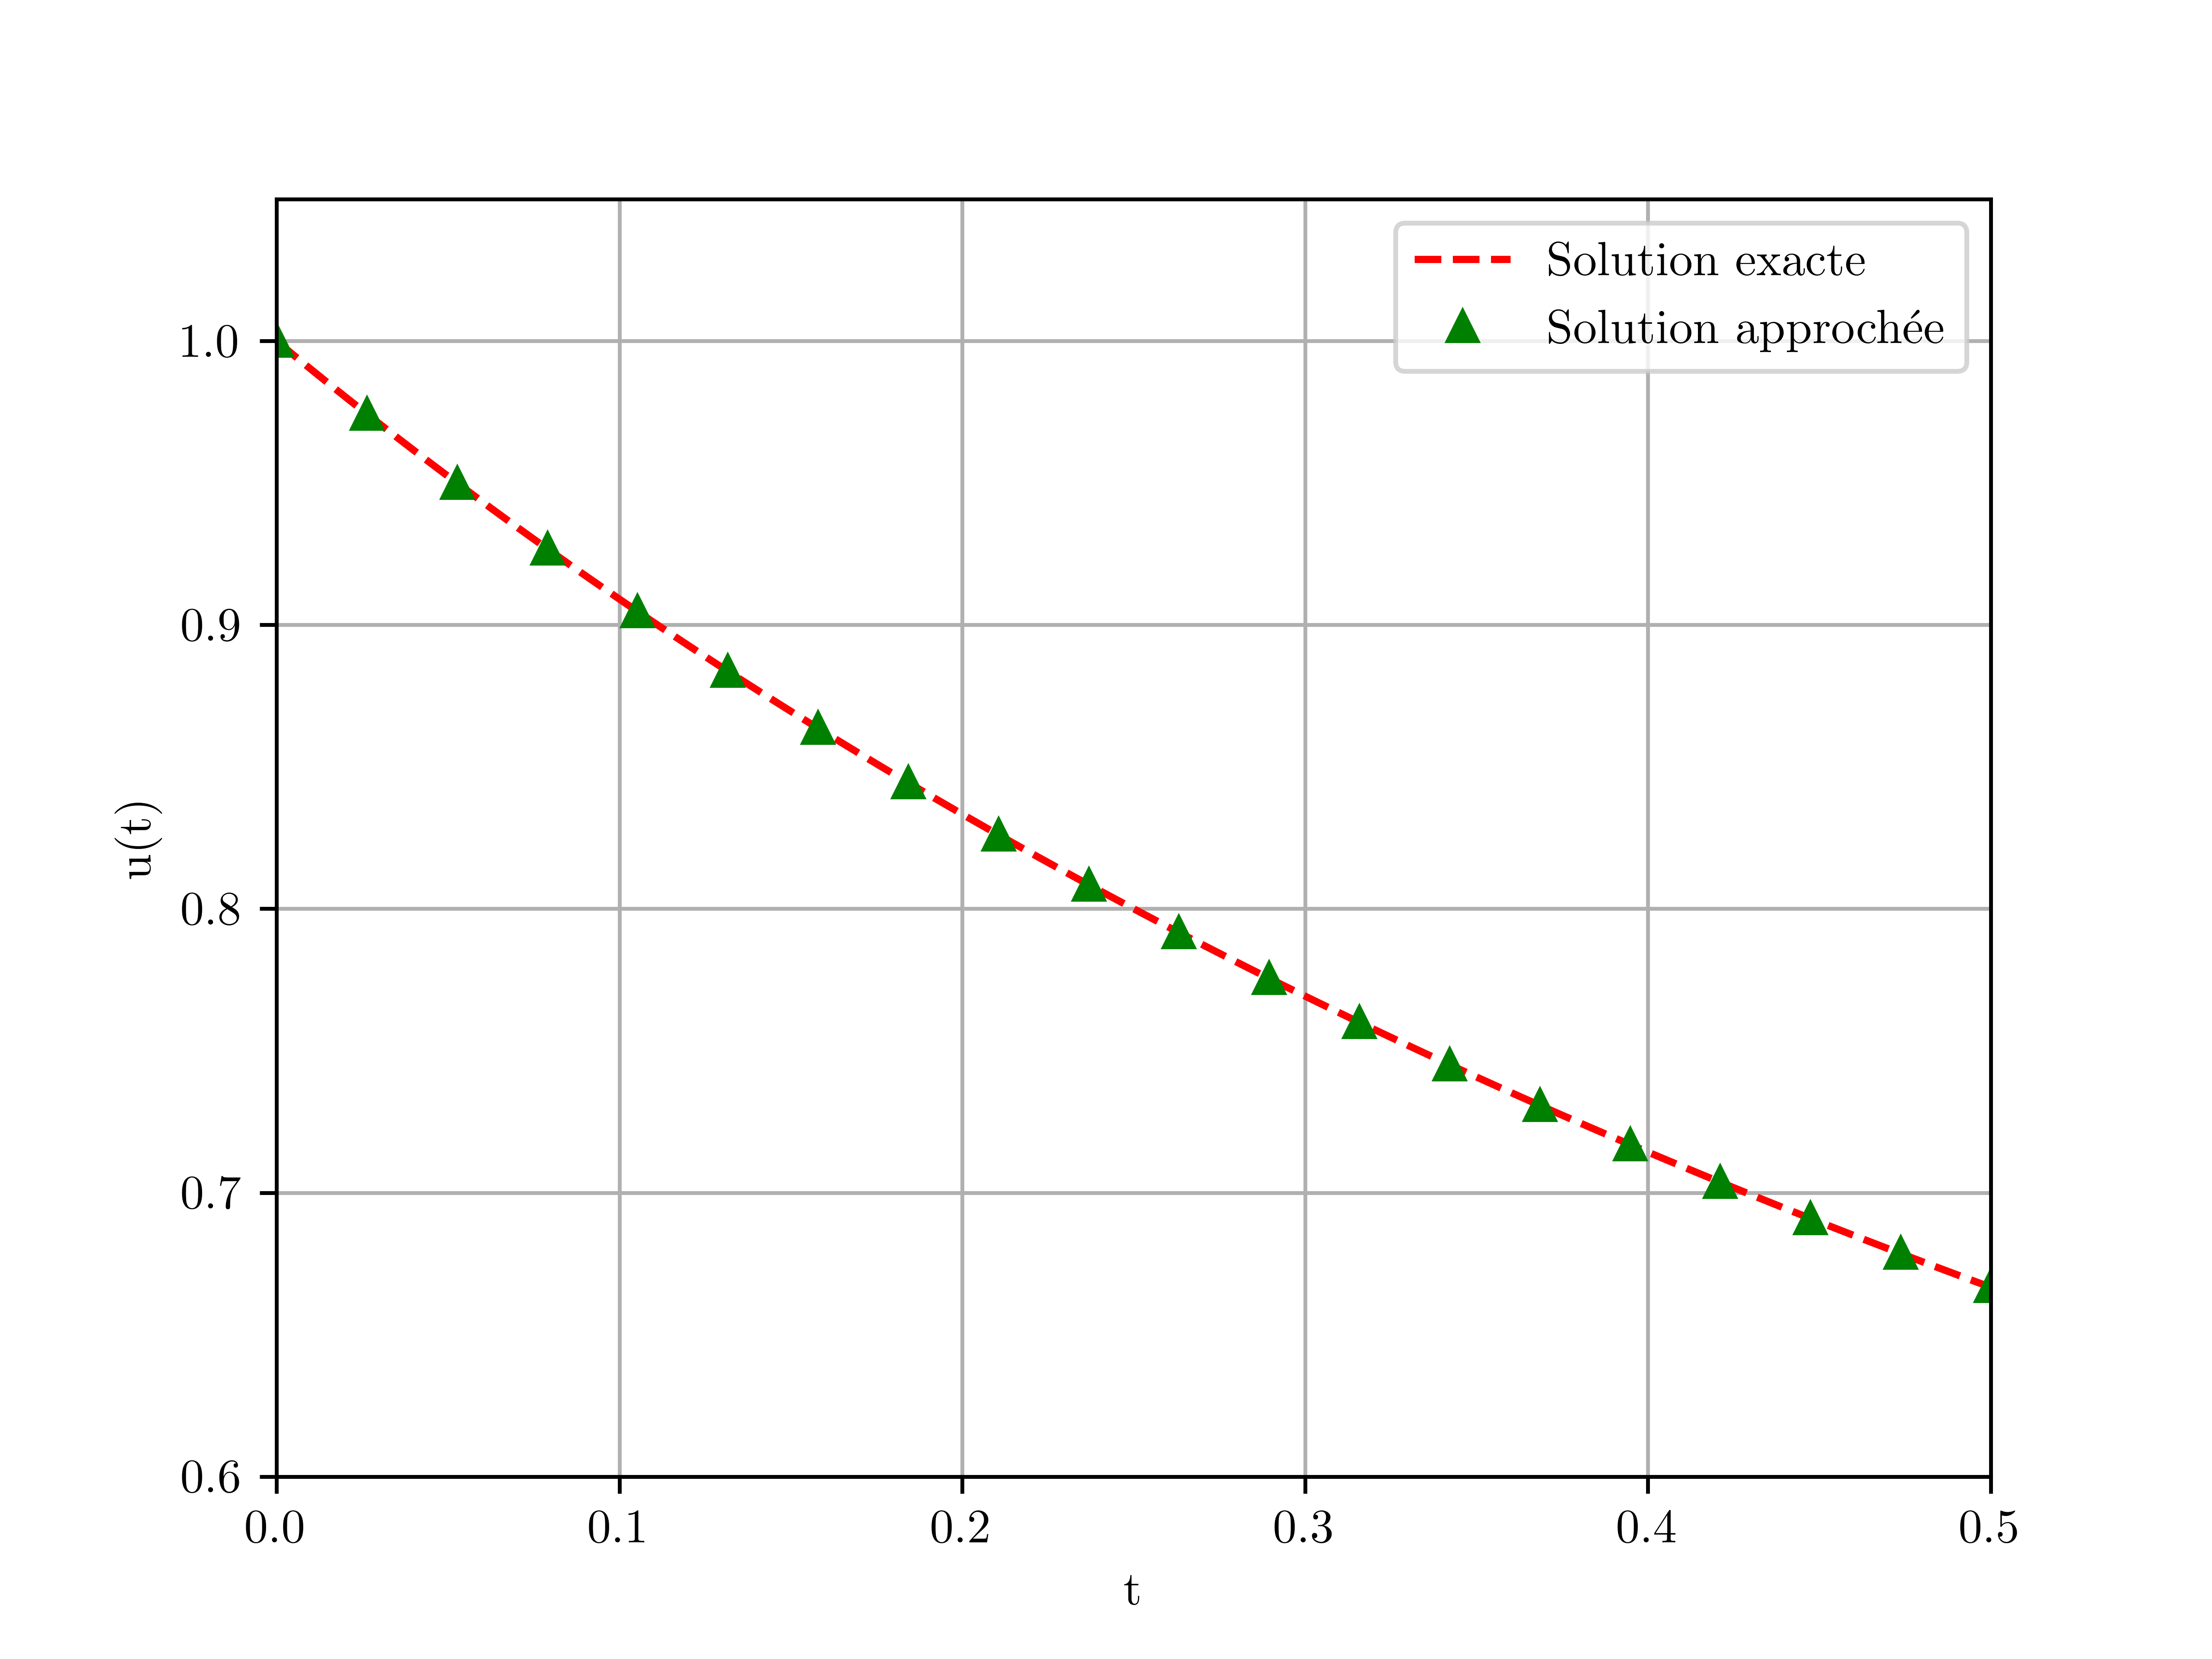
\includegraphics[scale = 0.5]{PolyU Presentation/images/plot.png}
\end{figure}
\end{frame}


\begin{frame}{Application de la méthode aux équations différentielles ordinaires}
    \textbf{Application: Exemple 2} \\
    Maintenant, nous allons considérer l'équation de Lane-Emden suivante:
\begin{equation}\label{ex:EDO_2}
    \begin{cases}
        u''(x)+\frac{2}{x}u'(x)+u(x) = x^5 + 30x^3,\\
        u(0) = u'(0)=0,
    \end{cases}
\end{equation}
où la solution exacte est exprimée par:
\begin{equation}
    u(x)=x^5.
\end{equation}
\end{frame}


\begin{frame}{Application de la méthode aux équations différentielles ordinaires}
     La méthode de perturbation d'Homotopie, implique :
\begin{equation} \label{sol:EDO_2}
    \left(v''+\frac{2}{x}v'\right) - \left(u''_0+\frac{2}{x}u'_0 \right) = p\left(x^5+30x^3-v-u''_0 - \frac{2}{x}u'_0\right).
\end{equation}
La solution de l'équation \ref{ex:EDO_2} est sous la forme:
\begin{equation}
    v=v_0+pv_1+p^2v_2+p^3v_3 + ...
\end{equation}
\end{frame}


\begin{frame}{Application de la méthode aux équations différentielles ordinaires}
\begin{align*}
    \begin{cases}
        &p^0 : v_0(x) = u_0(x)=0,\\
        &p^1 : v_1(x)=\frac{1}{56}x^7 + x^5,\\
        &p^2 : v_2(x) = -\frac{1}{5040}x^9 - \frac{1}{56}x^7,\\
        &p^3 : v_3(x) = \frac{1}{665280}x^{11}+\frac{1}{5040}x^9,\\
        &p^4 : v_4(x) = \frac{1}{121080960} x^{13} - \frac{1}{665280}x^{11},\\
        &p^5 : v_5(t) = \frac{1}{29059430400}x^{15} + \frac{1}{121080960} x^{13},\\
        &    .\\
        &    .\\
        &    .\\
    \end{cases}
\end{align*}
\end{frame}


\begin{frame}{Application de la méthode aux équations différentielles ordinaires}
    Finalement, la solution approchée le d'équation \ref{ex:EDO_2} est donnée par:
\begin{equation}
    u(x)=\lim_{p\to 1} v(x)=v_0(x)+v_1(x)+v_2(x)+...
\end{equation}
\end{frame}


\begin{frame}{Application de la méthode aux équations différentielles ordinaires}
    \begin{figure}[H]
    \centering
    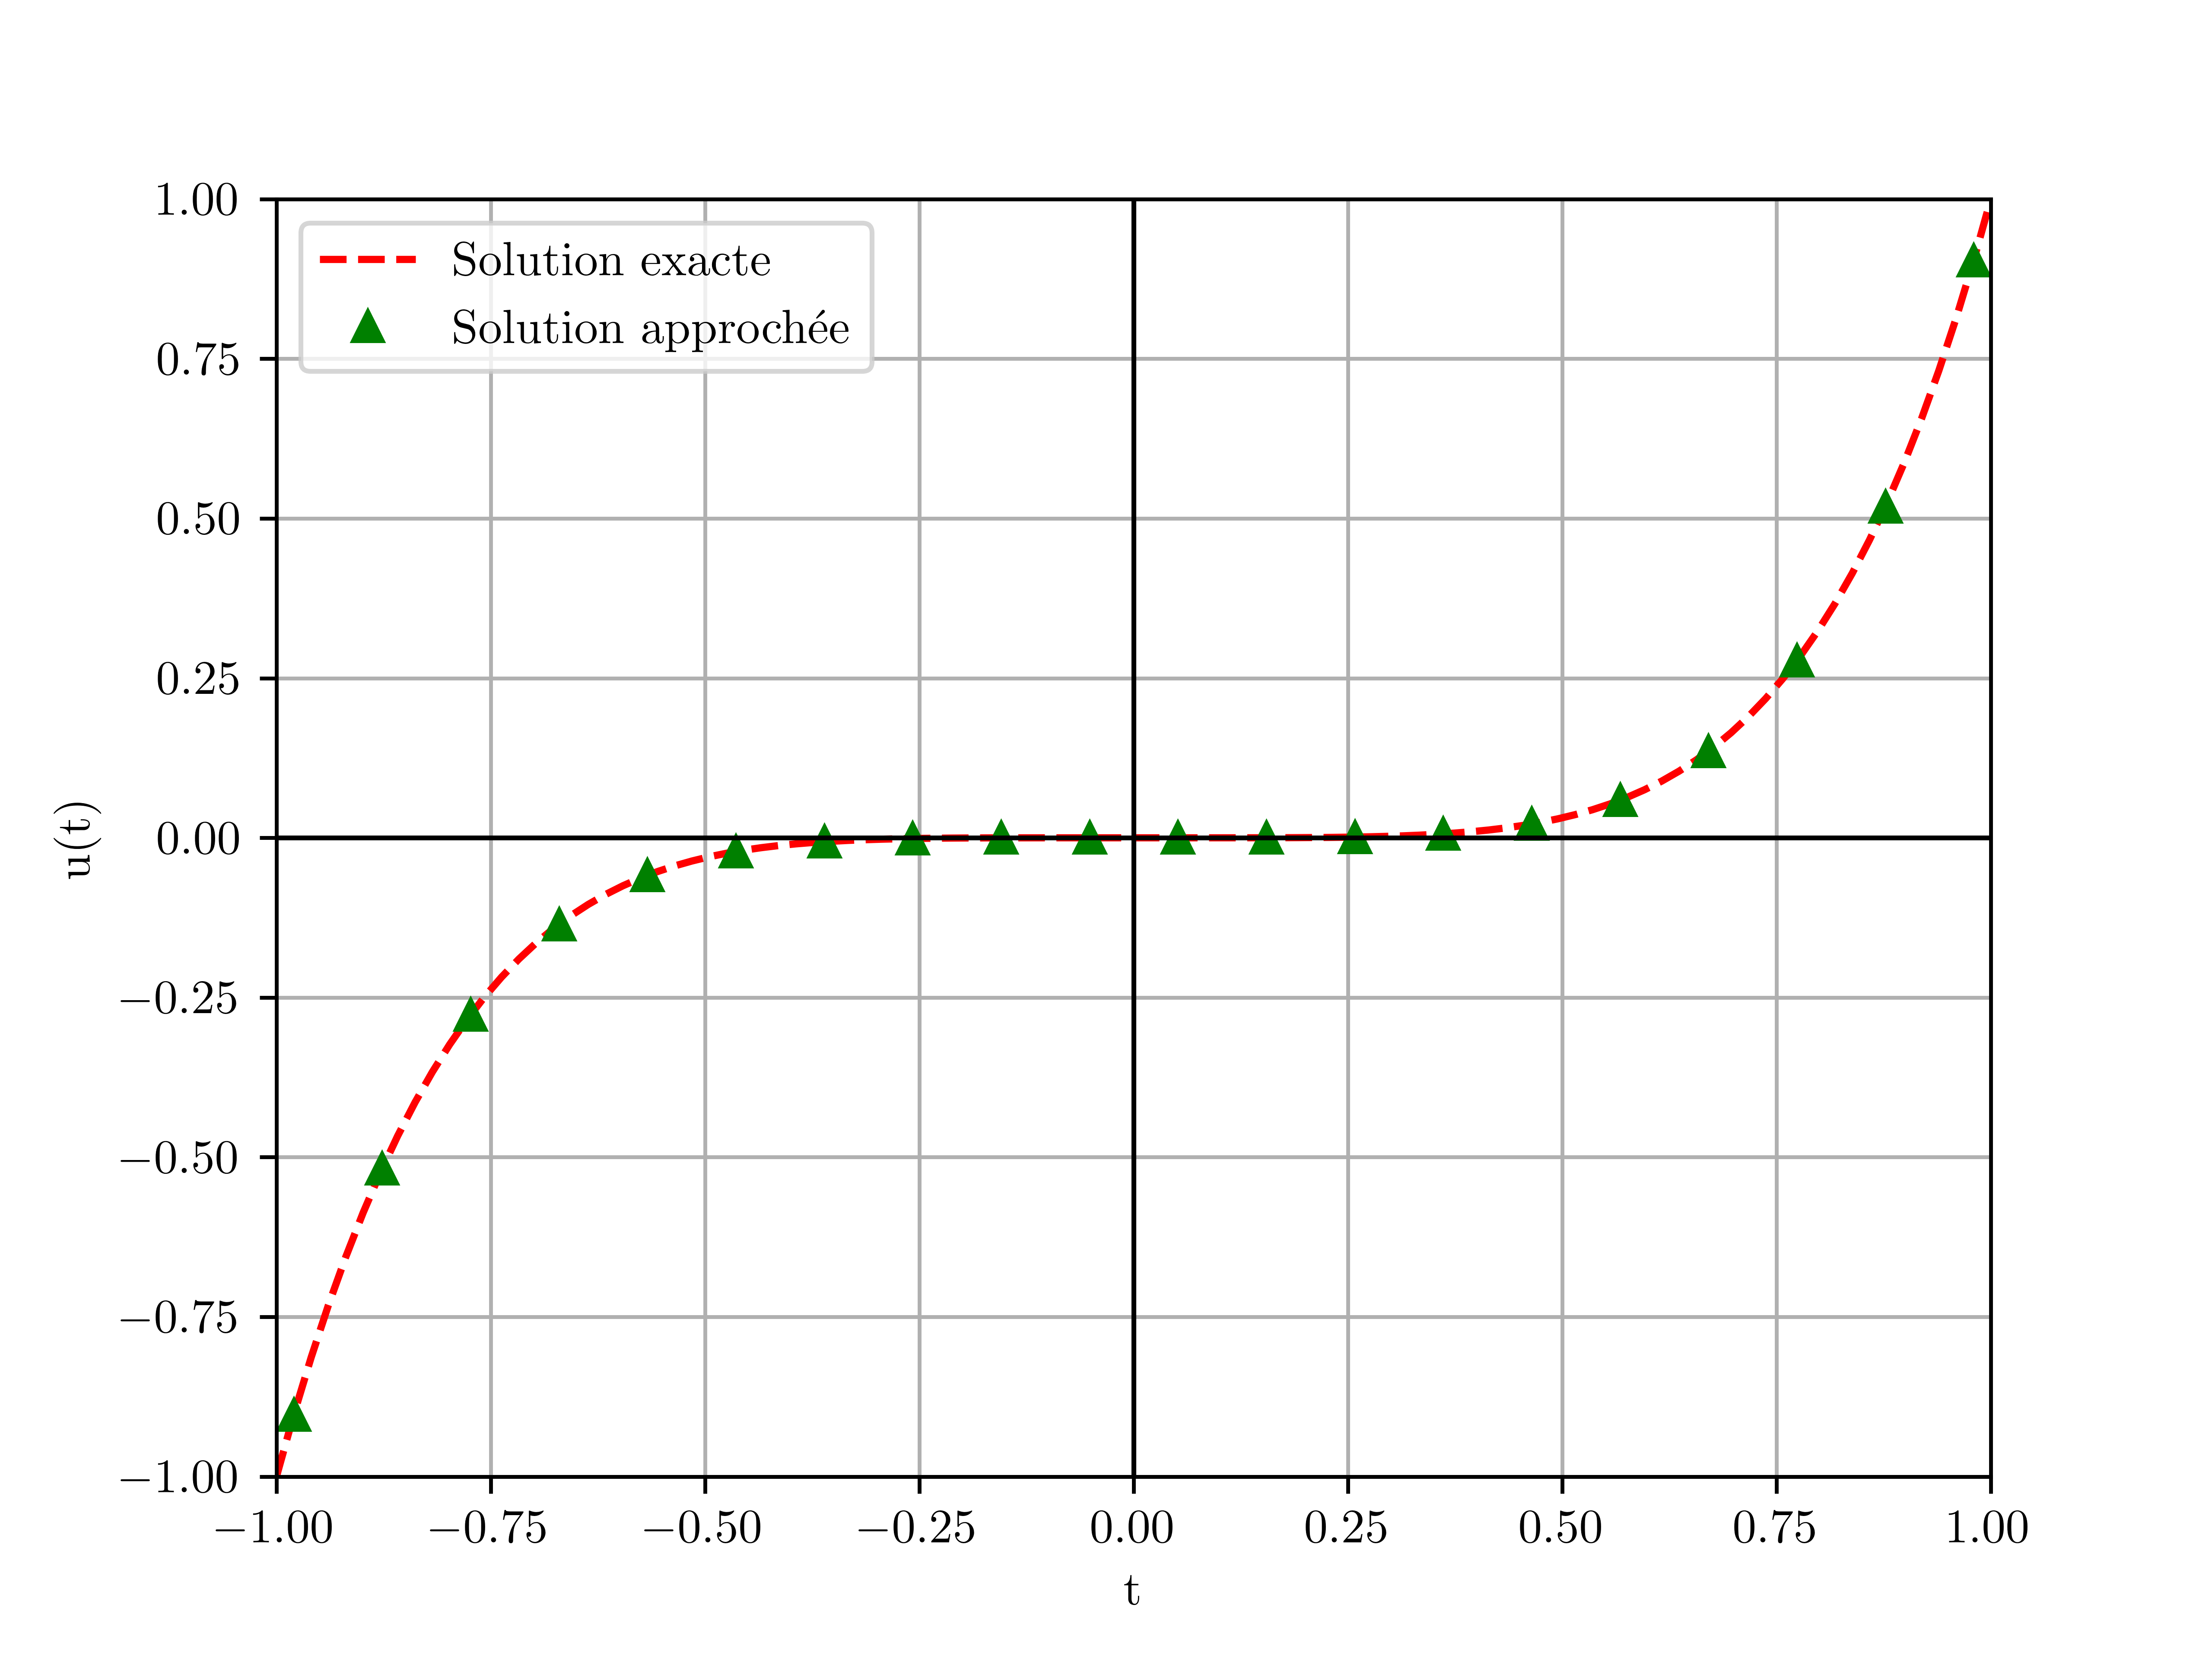
\includegraphics[scale = 0.5]{PolyU Presentation/images/plot (2).png}
\end{figure}
\end{frame}





\begin{frame}{Application de la méthode aux équations différentielles fractionnaires}
    \textbf{Description de la méthode}:
     Le problème de valeur initiale d'équations différentielles fractionnaires est donnée par sa forme opérationnelle:
 \begin{align}\label{eq: HMP_EDF_theorie}
     D^{\alpha} f(t) + Lf(t) = g(t)\\
     f^{(i)} (0) = c_i, \hspace{1cm} i=0,1,2, ..., n-1
 \end{align}
 où $c_i$ est la condition initial, $L$ désigne un opérateur linéaire qui peut inclus d'autre opérateurs de dérivées fractionnaires $D^{\beta}(\beta < \alpha)$ et $g$ est une fonction connue.
\end{frame}


\begin{frame}{Application de la méthode aux équations différentielles fractionnaires}
L'homotopie de l'équation \ref{eq: HMP_EDF_theorie} satisfait :
  \begin{equation}\label{eq:HPM_FDE_1}
      (1-p)D^{\alpha} f +p\left[ D^{\alpha}f + Lf(t) -g(t)\right]=0, \hspace{1cm} p\in [0,1],
  \end{equation}
  où
  \begin{equation}\label{eq:HPM_FDE_2}
      D^{\alpha}f+p\left[Lf(t)-g(t)\right]=0,
  \end{equation}
  avec $p\in[0,1]$ est un paramètre d'homotopie. Si $p=0$, l'équation \ref{eq:HPM_FDE_1} et \ref{eq:HPM_FDE_2} devient:
  \begin{equation}
      D^{\alpha} f=0
  \end{equation}
  Si $p=1$, les deux équations \ref{eq:HPM_FDE_1} et \ref{eq:HPM_FDE_2} donnent l'EDF original \ref{eq: HMP_EDF_theorie}.\\
\end{frame}


\begin{frame}{Application de la méthode aux équations différentielles fractionnaires}
La solution de l'équation \ref{eq: HMP_EDF_theorie} est:
  \begin{equation} \label{eq:sol_HPM_theorie}
      f(t)=f_0(t)+pf_1(t)+p^2f_2(t)+p^3f_3(t) + ...
  \end{equation}
    Substituons l'équation \ref{eq:sol_HPM_theorie} dans l'équation \ref{eq:HPM_FDE_2} et identifions les termes de même puissance de $p$, il vient:
  \begin{align*}
  \begin{cases}
            & p^0 : D^{\alpha} f_0 = 0\\
      & p^1 : D^{\alpha} f_1 = -Lf_0 + g(t)\\
      & p^2 : D^{\alpha} f_2 = -Lf_1(t)\\
      & p^3 : D^{\alpha} f_3 = -Lf_2(t)\\
      & .\\
      & .\\
  \end{cases}
  \end{align*}
\end{frame}

\begin{frame}{Application de la méthode aux équations différentielles fractionnaires}
    on peut réécrit les termes de solution de perturbation d'homotopie par :
\begin{align*}
    \begin{cases}
        & f_0 = \sum_{i=0}^{m-1} f^{(i)}(0) \frac{t^i}{i!} = \sum _{i=0}^{m-1} c_i \frac{t^i}{i!} \\
          & f_1 = -I^{\alpha} [Lf_0(t)] + I^{\alpha}[Lg(t)]\\
          & f_2 = -I^{\alpha}[Lf_1(t)]\\
          & f_3 = -I^{\alpha}[Lf_2(t)]\\
          & .\\
          & .\\
    \end{cases}
  \end{align*}
\end{frame}

 \begin{frame}{Application de la méthode aux équations différentielles fractionnaires}
     La forme générale de la solution HPM est donné par :
\begin{equation}
    f_n=-I^{\alpha}[Lf_{n-1}(t)]
\end{equation}
Alors la solution de perturbation d'homotopie est :
\begin{equation}
    f(t)=f_0+f_1+f_2+f_3 + ... +f_n + ...
\end{equation}
 \end{frame}

\begin{frame}{Application de la méthode aux équations différentielles fractionnaires}
    \textbf{Application: Exemple 1}
    Considérons l'équation différentielle fractionnaire linéaire suivante:
\begin{equation}
    \begin{cases}\label{ex:EDF_1}
        D^{\alpha}x(t) + x(t) = \frac{2}{\Gamma(3-\alpha)} t^{2-\alpha} + t^3,\\
        x(0)=0,\\
        x'(0)=0.
    \end{cases}
\end{equation}
où la solution exacte pour $\alpha = 1,9$ est donnée par:
\begin{equation}
    x(t)=t^2.
\end{equation}
\end{frame}


\begin{frame}{Application de la méthode aux équations différentielles fractionnaires}
    On construit l'homotopie suivante:
\begin{equation} \label{eq:HPM_EDF1}
    D^{\alpha} x(t) +p\left[x(t)-\frac{2}{\Gamma(3-\alpha)}t^{2-\alpha}-t^3\right] =0, \hspace{1cm} t\in \Omega,
\end{equation}
La solution de \ref{ex:EDF_1} peut être exprimée comme suit :
\begin{equation}\label{sol:EDF_1}
    x(t) =x_0(t) + px_1(t) + p^2x_2(t) + ... = \sum _{i=0}^{\infty} p^i x_i(t)
\end{equation}
 il vient :
\begin{align*}
    \sum_{i=0}^{\infty} D^{\alpha} p^{(i)} x_i(t) = -p\left[\sum_{i=0}^{\infty} p^{(i)} x_i(t) -\frac{2}{\Gamma(3-\alpha)} t^{2-\alpha} -t^3\right]
\end{align*}
\end{frame}

\begin{frame}{Application de la méthode aux équations différentielles fractionnaires}
\begin{align} \label{eq:p_1}
    \begin{cases}
    & p^0 : D^{\alpha}x_0(t)=0, \\
    & p^1 : D^{\alpha}x_1(t) = -x_0(t) + \frac{2}{\Gamma(3-\alpha)} t^{2-\alpha} + t^3,\\
    & p^2 : D^{\alpha} x_2(t) = -x_1(t),\\
    & p^3 : D^{\alpha} x_3(t) = -x_2(t),\\
    &     . \\
    &     .\\
    &     .\\
    \end{cases}
\end{align}
\end{frame}

\begin{frame}{Application de la méthode aux équations différentielles fractionnaires}
    Appliquent l'opérateur $I^{\alpha}$ sur les deux cotés de d'équations \ref{eq:p_1} et on utilisons les propriétés de L'intégrale fractionnaire de Riemann-Liouville d'ordre $\alpha \geq 0$, on obtient 
    \begin{align*}
    &x _0(t)=0\\
    & x_1(t) = \frac{2}{\Gamma(3-\alpha)}t^{2-\alpha} + t^3\\
    & x_2(t) = -\frac{2}{\Gamma(3-\alpha)} t^{2-\alpha} -t^3\\
    & x_3(t) = \frac{2}{\Gamma(3+2\alpha)}t^{2+2\alpha} + \frac{6}{\Gamma(3+3\alpha)} t^{3+3\alpha} \\
    & .\\
    & .\\
    \end{align*}
\end{frame}


\begin{frame}{Application de la méthode aux équations différentielles fractionnaires}
    Donc la solution de l'équation \ref{ex:EDF_1} est donnée par:
\begin{align*}
        x(t) &= x_0(t) + px_1(t) + p^2x_2(t) + p^3x_3(t)+...\\
        & = 0 + t^2 + \frac{\Gamma(4)}{\Gamma(4+\alpha)} -\frac{2}{\Gamma(3+\alpha)} t^{2+\alpha} -\frac{6}{\Gamma(4+2\alpha)} t^{3+2\alpha} + \frac{2}{\Gamma(3+2\alpha)}t^{2+2\alpha} +...
\end{align*}
si $\alpha = 1,9$
\begin{align*}
    x(t) &= t^2 + \frac{6}{\Gamma(5,9)}t^{4,9} -\frac{2}{\Gamma(4,9)}t^{3,9} - \frac{6}{\Gamma(7,8)}t^{6,8} + ...\\
    &= t^2 + 0.059247439t^{4,9} - 0.096770806t^{3,9} - 0.001776766299 t^{6,8} + ...\\
    & \approx t^2
\end{align*}
\end{frame}


\begin{frame}{Application de la méthode aux équations différentielles fractionnaires}
    \begin{figure}[H]
    \centering
    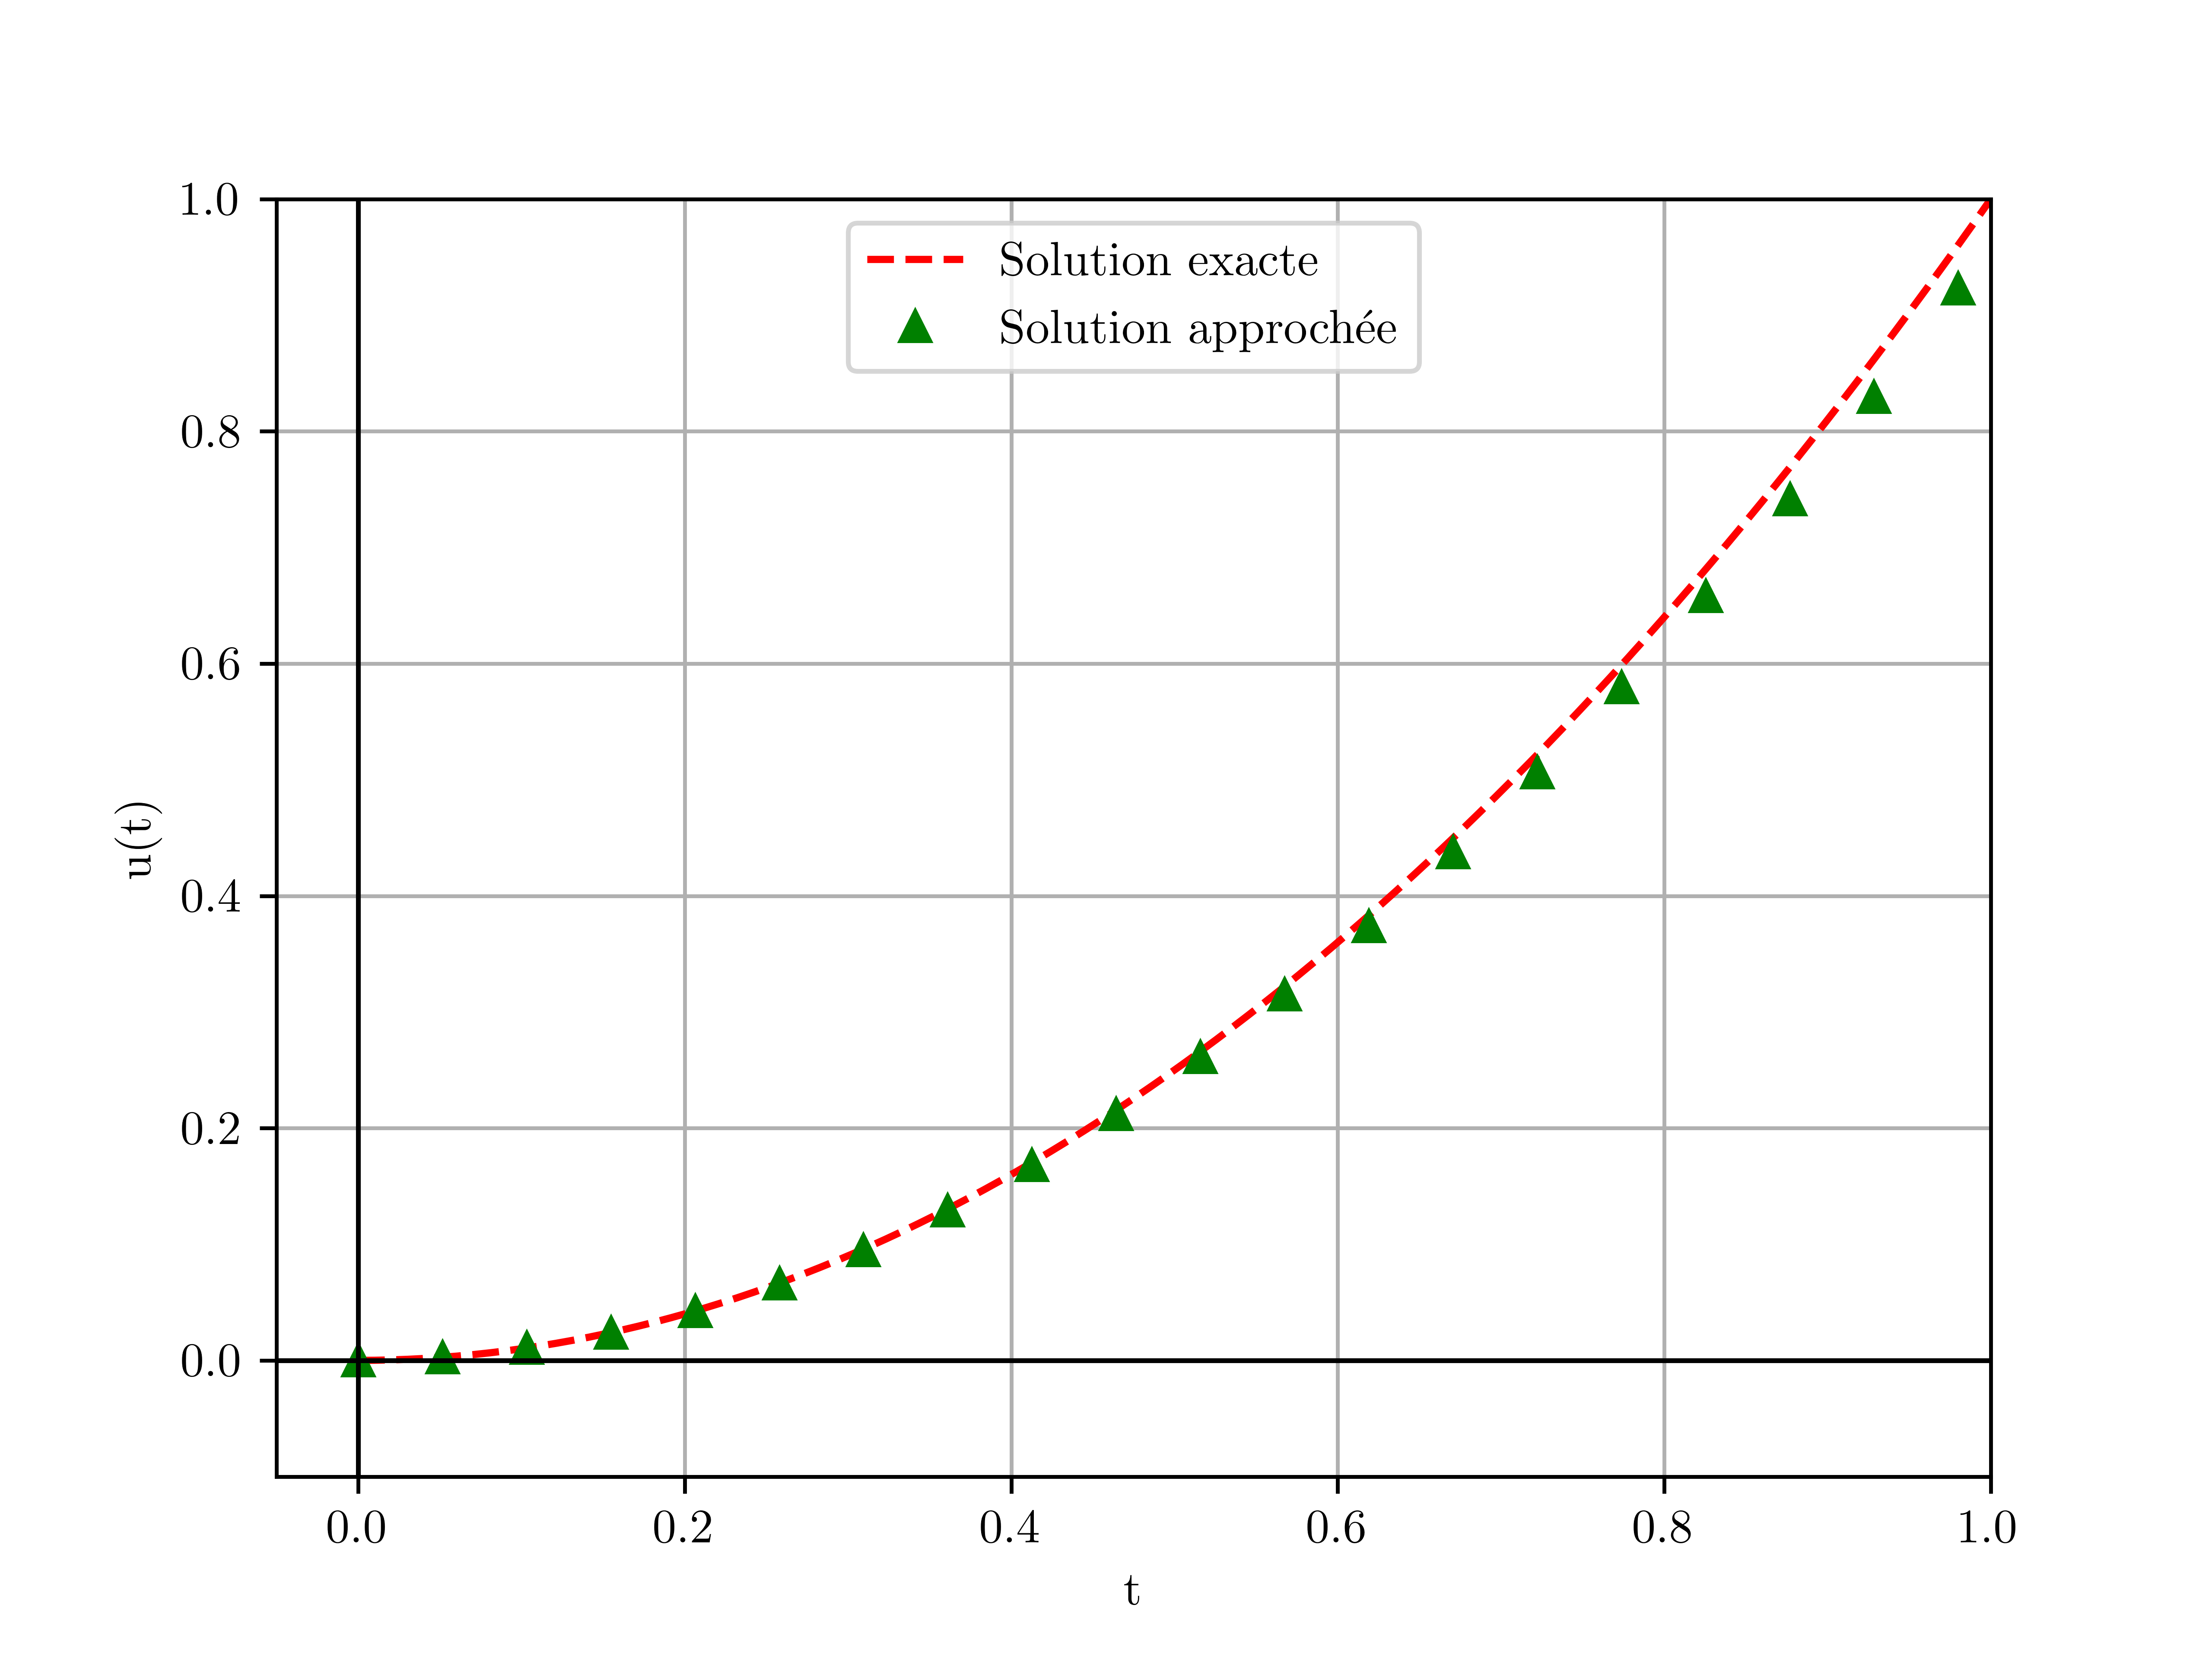
\includegraphics[scale = 0.5]{PolyU Presentation/images/plot (3).png}
\end{figure}
\end{frame}

\begin{frame}{Application de la méthode aux équations
différentielles fractionnaires}
    \begin{table}[H]\label{tab:1}
\begin{tabular*}{\textwidth}{llll}
$\mathbf{t_k}$ & \textbf{Solution exacte} & \textbf{Solution Approchée}  & \textbf{Erreur} $\mathbf{= |x(t)-x(t)|}$    \\ 
\hline
0.0   & 0    & 0          & 0                 \\
0.1   & 0.10 & 0.00998856 & 0.09001144 \\
0.2   & 0.04 & 0.0398404  & 0.0001596  \\
0.3   & 0.09 & 0.0892778  & 0.0007222 \\
0.4   & 0.16 & 0.157946   & 0.0007222 \\
0.5   & 0.25 & 0.245486   & 0.004514 \\
0.6   & 0.36 & 0.351595   & 0.008405 \\
0.7   & 0.49 & 0.476084   & 0.013916  \\
0.8   & 0.64 & 0.618931   & 0.021069 \\
0.9   & 0.81 & 0.780324   & 0.029676 \\
1     & 1.00 & 0.9607     & 0.0393 \\
\hline
\end{tabular*}
\end{table}
\end{frame}






\begin{frame}{Application de la méthode aux équations différentielles fractionnaires}
    \textbf{Application : Exemple 2}
    Maintenant, considérons la deuxième équation différentielle factionnaire linéaire suivante :
\begin{equation}\label{ex:EDF_2}
    \begin{cases}
        D^{\alpha} x(t) +x(t) = 1\\
        x(0)=0\\
        x'(t) =0
    \end{cases}
\end{equation}
où la solution exacte pour $\alpha = 1.1$ est donnée par:
\begin{equation}
    x(t)=t^{1,1} E_{1,1. 2,1} (-t^{1,1})
\end{equation}
\end{frame}


\begin{frame}{Application de la méthode aux équations différentielles fractionnaires}
    On construit l'homotopie suivante:
\begin{equation} \label{eq:HPM_EDF2}
    D_{\alpha} x(t) +p\left[x(t)-1\right]=0
\end{equation}
La solution de \ref{ex:EDF_1} peut être exprimée comme suit :
\begin{equation}\label{sol:EDF_2}
    x=x_0 + px_1 + p^2x_2 ... = \sum _{i=0}^{\infty} p^i x_i
\end{equation}
il vient :
\begin{align*}
    \sum_{i=0}^{\infty} D^{\alpha} p^{(i)}x_i(t) = p\left(1-\sum_{i=0}^{\infty} p^{i}x_i (t) \right)
\end{align*}
\end{frame}

\begin{frame}{Application de la méthode aux équations différentielles fractionnaires}
    \begin{align}\label{eq:p_2}
\begin{cases}
    & p^0 : D^{\alpha}x_0(t)=0, \\
    & p^1 : D^{\alpha}x_1(t) = 1 -x_0(t),\\
    & p^2 : D^{\alpha} x_2(t) = -x_1(t),\\
    & p^3 : D^{\alpha} x_3(t) = -x_2(t),\\
    &     . \\
    &     .\\
    &     .\\
\end{cases}
\end{align}
\end{frame}

\begin{frame}{Application de la méthode aux équations différentielles fractionnaires}
    On obtient 
    \begin{align*}
    & x_0(t) = 0\\
    & x_1(t) = \frac{t^{\alpha}}{\Gamma(\alpha +1)}\\
    & x_2(t) = -\frac{t^{2\alpha}}{\Gamma(2\alpha +1)}\\
    & x_3(t) = \frac{t^{3\alpha}}{\Gamma(3\alpha+1)}\\
    & . \\
    & . \\
\end{align*}
\end{frame}

\begin{frame}{Application de la méthode aux équations différentielles fractionnaires}
    Donc la solution de l'équation \ref{ex:EDF_2} est donnée par:
\begin{align*}
        x(t) &= x_0(t) + px_1(t) + p^2x_2(t) + p^3x_3(t)+...\\
        &= \sum_{K=1}^{\infty}(-1)^{k+1}\frac{t^{k\alpha}}{\Gamma(k\alpha +1)}
\end{align*}
si $\alpha = 1,1$
\begin{align*}
    x(t) &= \frac{t^{1,1}}{\Gamma(2,1)} - \frac{t^{2,2}}{\Gamma(3,2)} +\frac{t^{3,3}}{\Gamma(4,3)} - \frac{t^{4,4}}{\Gamma(5,4)}+...\\
    &= \frac{t^{1,1}}{0.95135} - \frac{t^{2,2}}{0,95135} +\frac{t^{3,3}}{0.95135} - \frac{t^{4,4}}{0.95135}+...\\
    & = 0.95557t^{1,1} - 0.41255t^{2,2} + 0.11293t^{3,3}- 0.02242 t^{4,4} + ...
\end{align*}
\end{frame}

\begin{frame}{Application de la méthode aux équations différentielles fractionnaires}
    \begin{figure}[H]
    \centering
    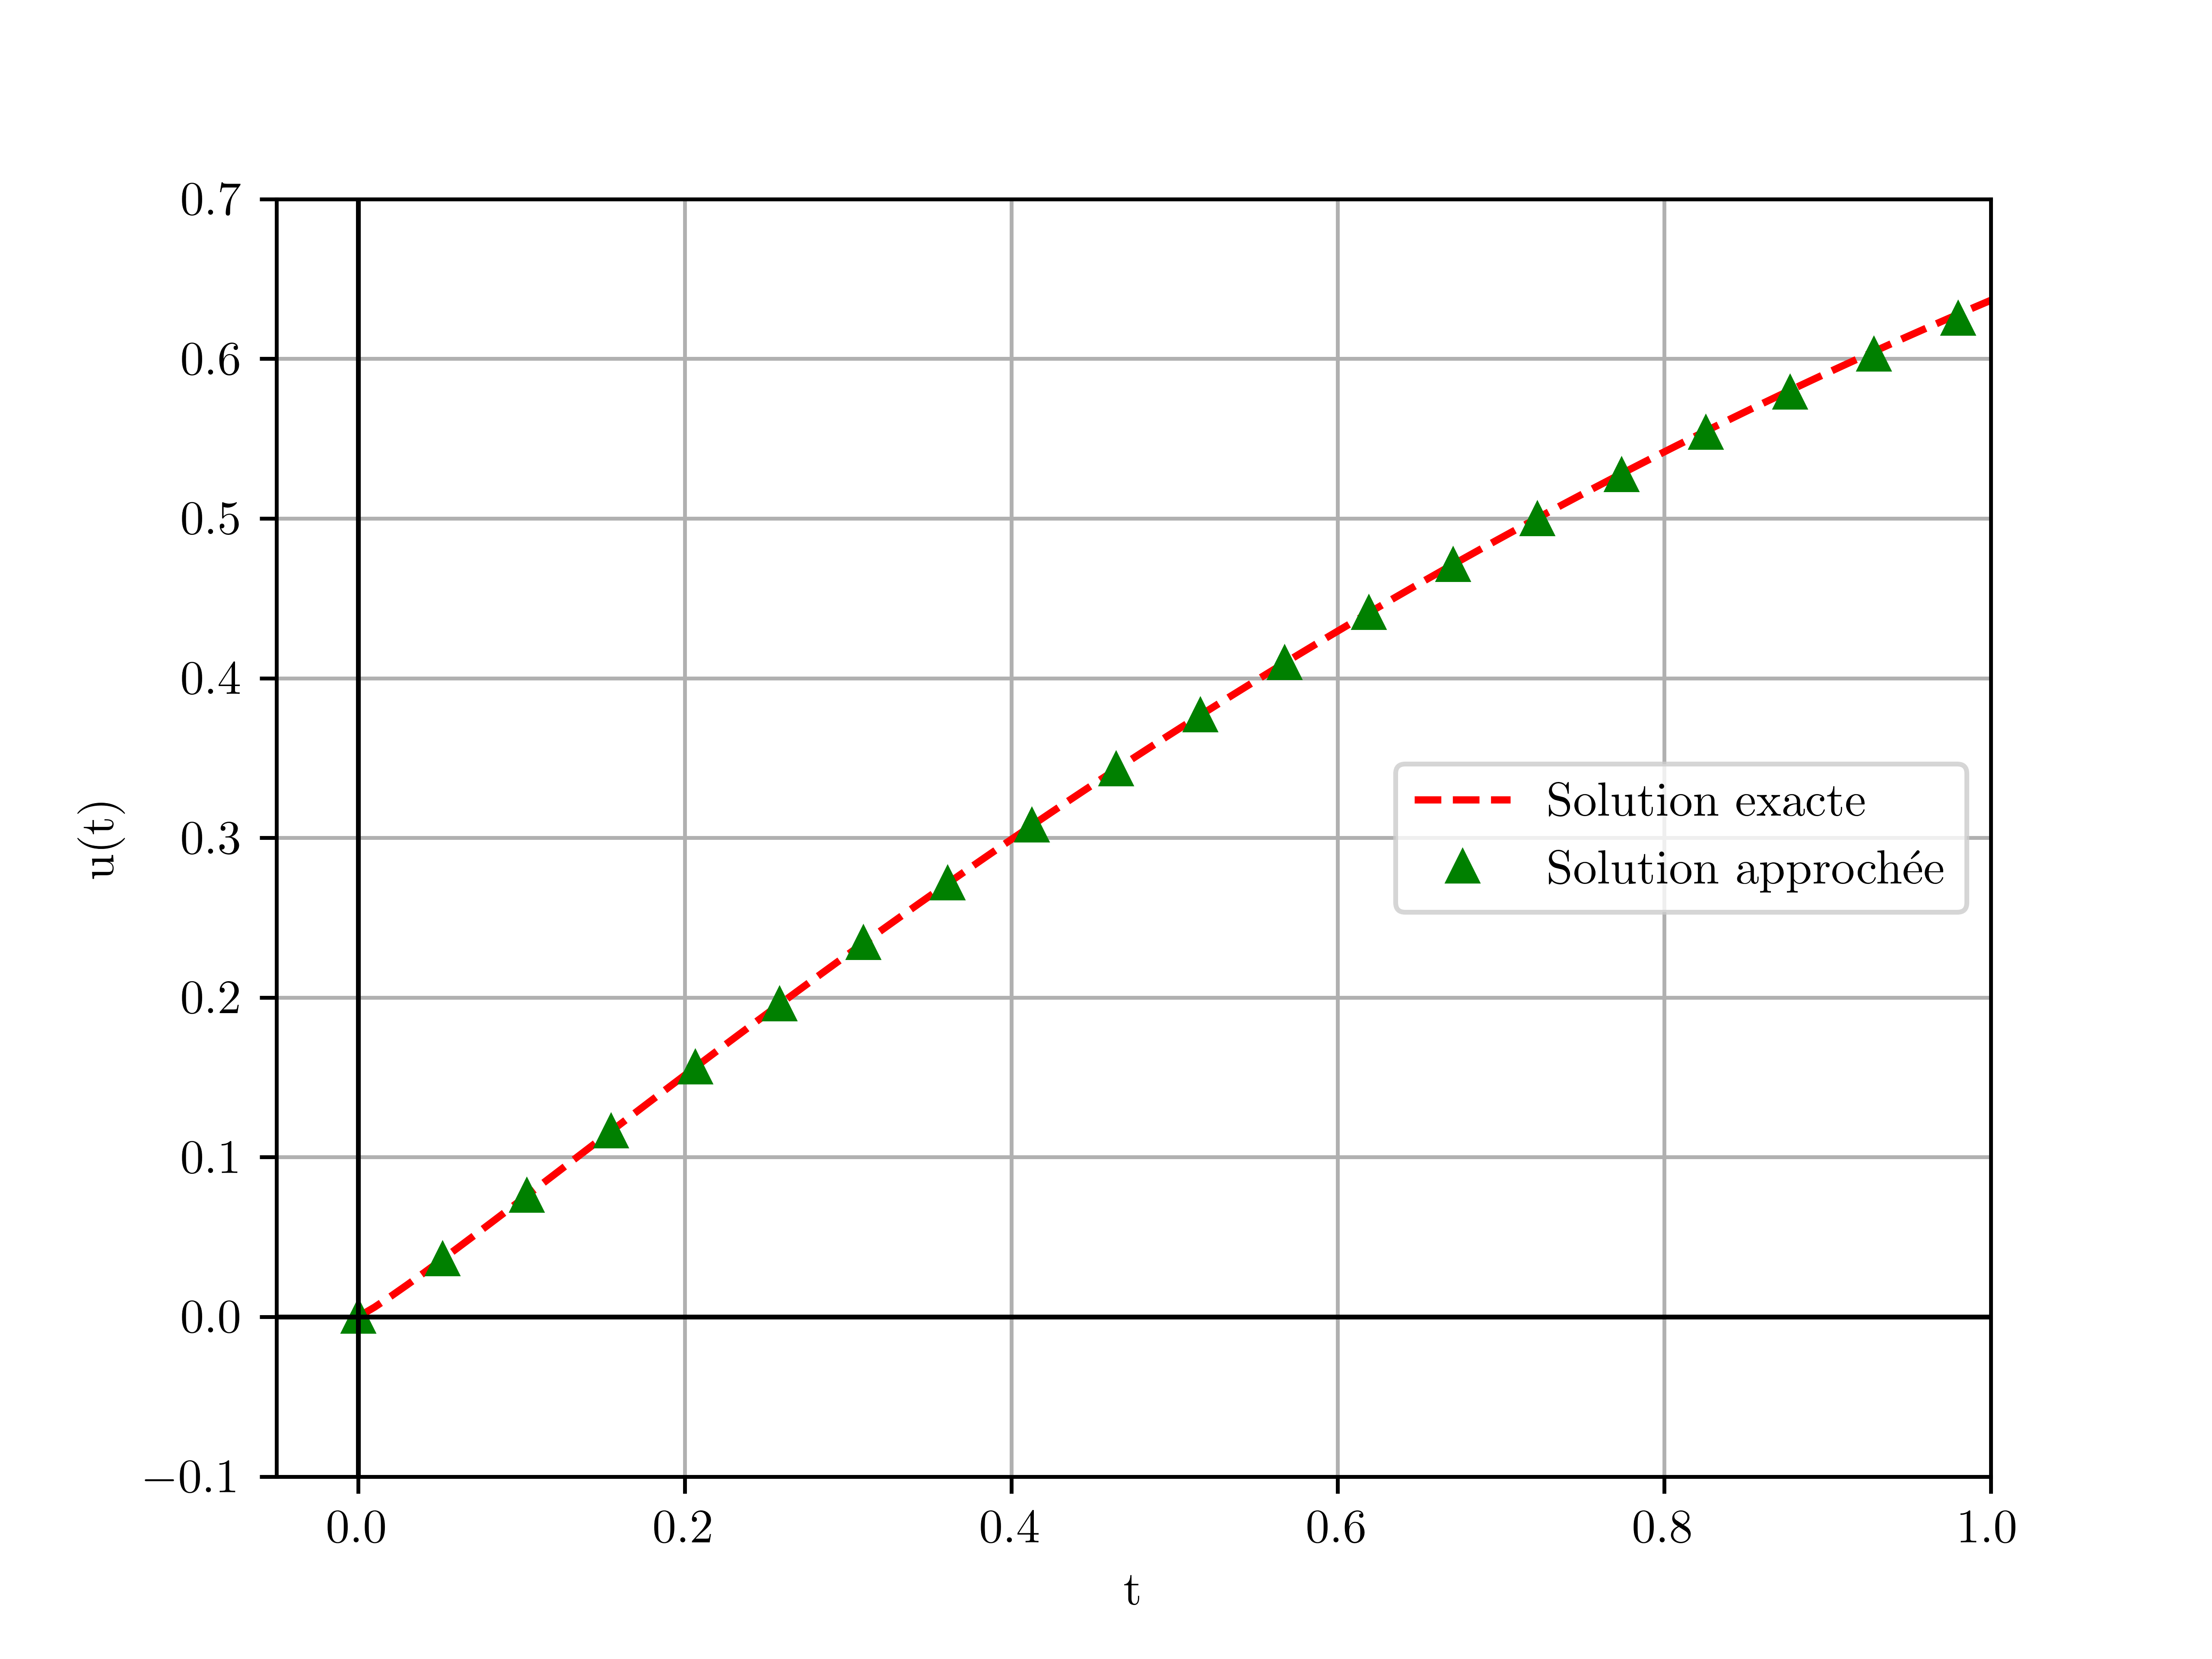
\includegraphics[scale = 0.5]{PolyU Presentation/images/plot (6).png}
\end{figure}
\end{frame}

\begin{frame}{Application de la méthode aux équations différentielles fractionnaires}
\begin{table}[H] \label{tab:2} 
\begin{tabular*}{\linewidth}{llll}
$\mathbf{t_k}$ & \textbf{Solution exacte} & \textbf{Solution Approchée} & \textbf{Erreur}    \\ 
\hline
0.0  &  0                  &  0                  &  0                \\
0.1  &  0.073357053781371  &  0.0733563  &  7.53781371$\times$10$^{-7}$\\
0.2  &  0.151282884629052  &  0.151281   &  1.884629052$\times$10$^{-6}$ \\
0.3  &  0.226984580680193  &  0.226982   &  2.58068193$\times$10$^{-6}$ \\
0.4  &  0.29890238480688   &  0.298899   &  3.38480688$\times$10$^{-6}$ \\
0.5  &  0.366411147911488  &  0.366407   &  4.147911488$\times$10$^{-6}$ \\
0.6  &  0.429259300754372  &  0.429254   &  5.300754372$\times$10$^{-6}$\\
0.7  &  0.487372840288318  &  0.487367   &  5.840288318$\times$10$^{-6}$\\
0.8  &  0.540762298480572  &  0.540756   &  6.298480572$\times$10$^{-6}$\\
0.9  &  0.589469952960841  &  0.589464   &  5.952960841$\times$10$^{-6}$\\
1    &  0.633536032460000  &  0.63353    &  6.03246$\times$ 10$^{-6}$\\
\hline
\end{tabular*}
\end{table}
\end{frame}

\section{Conclusion}
\end{document}